%% abtex2-modelo-relatorio-tecnico.tex, v-1.9.7 laurocesar
%% Copyright 2012-2018 by abnTeX2 group at http://www.abntex.net.br/ 
%%
%% This work may be distributed and/or modified under the
%% conditions of the LaTeX Project Public License, either version 1.3
%% of this license or (at your option) any later version.
%% The latest version of this license is in
%%   http://www.latex-project.org/lppl.txt
%% and version 1.3 or later is part of all distributions of LaTeX
%% version 2005/12/01 or later.
%%
%% This work has the LPPL maintenance status `maintained'.
%% 
%% The Current Maintainer of this work is the abnTeX2 team, led
%% by Lauro César Araujo. Further information are available on 
%% http://www.abntex.net.br/
%%
%% This work consists of the files abntex2-modelo-relatorio-tecnico.tex,
%% abntex2-modelo-include-comandos and abntex2-modelo-references.bib
%%

% ------------------------------------------------------------------------
% ------------------------------------------------------------------------
% abnTeX2: Modelo de Relatório Técnico/Acadêmico em conformidade com 
% ABNT NBR 10719:2015 Informação e documentação - Relatório técnico e/ou
% científico - Apresentação
% ------------------------------------------------------------------------ 
% ------------------------------------------------------------------------

\documentclass[
  % -- opções da classe memoir --
  12pt,				% tamanho da fonte
  openright,			% capítulos começam em pág ímpar (insere página vazia caso preciso)
  twoside,			% para impressão em recto e verso. Oposto a oneside
  a4paper,			% tamanho do papel. 
  % -- opções da classe abntex2 --
  %chapter=TITLE,		% títulos de capítulos convertidos em letras maiúsculas
  %section=TITLE,		% títulos de seções convertidos em letras maiúsculas
  %subsection=TITLE,	% títulos de subseções convertidos em letras maiúsculas
  %subsubsection=TITLE,% títulos de subsubseções convertidos em letras maiúsculas
  % -- opções do pacote babel --
  english,			% idioma adicional para hifenização
  french,				% idioma adicional para hifenização
  spanish,			% idioma adicional para hifenização
  brazil,				% o último idioma é o principal do documento
  ]{abntex2}


% ---
% PACOTES
% ---
% ---- packs adicionais
\usepackage{lastpage}
\usepackage{xcolor}
\usepackage{listings}
\lstset{basicstyle=\ttfamily,
  showstringspaces=false,
  commentstyle=\color{red},
  keywordstyle=\color{blue}
}
\usepackage{hyperref}
\usepackage{caption}
\usepackage{subcaption}
\usepackage{adjustbox}
\usepackage{etoolbox}

% ---
% Pacotes fundamentais 
% ---
\usepackage{lmodern}			% Usa a fonte Latin Modern
\usepackage[T1]{fontenc}		% Selecao de codigos de fonte.
\usepackage[utf8]{inputenc}		% Codificacao do documento (conversão automática dos acentos)
\usepackage{indentfirst}		% Indenta o primeiro parágrafo de cada seção.
\usepackage{color}				% Controle das cores
\usepackage{graphicx}			% Inclusão de gráficos
\usepackage{microtype} 			% para melhorias de justificação
% ---

% ---
% Pacotes adicionais, usados no anexo do modelo de folha de identificação
% ---
\usepackage{multicol}
\usepackage{multirow}
% ---
  
% ---
% Pacotes adicionais, usados apenas no âmbito do Modelo Canônico do abnteX2
% ---
\usepackage{lipsum}				% para geração de dummy text
% ---

% ---
% Pacotes de citações
% ---
\usepackage[brazilian,hyperpageref]{backref}	 % Paginas com as citações na bibl
\usepackage[ieeetr]{abntex2cite}	% Citações padrão ABNT

% --- 
% CONFIGURAÇÕES DE PACOTES
% --- 

% ---
% Configurações do pacote backref
% Usado sem a opção hyperpageref de backref
\renewcommand{\backrefpagesname}{Citado na(s) página(s):~}
% Texto padrão antes do número das páginas
\renewcommand{\backref}{}
% Define os textos da citação
\renewcommand*{\backrefalt}[4]{
  \ifcase #1 %
    Nenhuma citação no texto.%
  \or
    Citado na página #2.%
  \else
    Citado #1 vezes nas páginas #2.%
  \fi}%
% ---

% ---
% Informações de dados para CAPA e FOLHA DE ROSTO
% ---
\titulo{Implementações práticas de DSP e RF com GNURadio e HackRF One}
\autor{Jefferson da Silva Cândido}
\local{Uberlândia, Minas Gerais}
\data{\the\year}
\instituicao{%
  Universidade Federal de Uberlândia -- UFU
  \par
  Faculdade de Engenharia Elétrica
  \par
  Graduação em Engenharia Eletrônica e de Telecomunicações}
\tipotrabalho{Trabalho de Conclusão de Curso}
% O preambulo deve conter o tipo do trabalho, o objetivo, 
% o nome da instituição e a área de concentração 
\orientador{Dr. Antônio Cláudio Paschoarelli Veiga}

\preambulo{Trabalho apresentado na Universidade Federal de Uberlândia como requisito para conclusão do curso de graduação em Engenharia Eletrônica e de Telecomunicações.}
% ---

% ---
% Configurações de aparência do PDF final

% alterando o aspecto da cor azul
\definecolor{blue}{RGB}{41,5,195}

% informações do PDF
\makeatletter
\hypersetup{
      %pagebackref=true,
    pdftitle={\@title}, 
    pdfauthor={\@author},
      pdfsubject={\imprimirpreambulo},
      pdfcreator={LaTeX with abnTeX2},
    pdfkeywords={abnt}{latex}{abntex}{abntex2}{relatório técnico}, 
    colorlinks=true,       		% false: boxed links; true: colored links
      linkcolor=blue,          	% color of internal links
      citecolor=blue,        		% color of links to bibliography
      filecolor=magenta,      		% color of file links
    urlcolor=blue,
    bookmarksdepth=4
}
\makeatother
% --- 

% --- 
% Espaçamentos entre linhas e parágrafos 
% --- 

% O tamanho do parágrafo é dado por:
\setlength{\parindent}{1.3cm}

% Controle do espaçamento entre um parágrafo e outro:
\setlength{\parskip}{0.2cm}  % tente também \onelineskip

% ---
% compila o indice
% ---
\makeindex
% ---

% ----
% Início do documento
% ----
\begin{document}

% Seleciona o idioma do documento (conforme pacotes do babel)
%\selectlanguage{english}
\selectlanguage{brazil}

% Retira espaço extra obsoleto entre as frases.
\frenchspacing

% ----------------------------------------------------------
% ELEMENTOS PRÉ-TEXTUAIS
% ----------------------------------------------------------
\pretextual

% ---
% Capa
% ---
\imprimircapa
% ---

% ---
% Folha de rosto
% (o * indica que haverá a ficha bibliográfica)
% ---
\imprimirfolhaderosto
% ---

% ---
% Anverso da folha de rosto:
% ---

% \begin{fichacatalografica}
%   \vspace*{15cm} % Posição vertical
%   \hrule % Linha horizontal
%   \begin{center} % Minipage Centralizado
%     \begin{minipage}[c]{12.5cm} % Largura
%       \imprimirautor
%       \hspace{0.5cm} \imprimirtitulo / \imprimirautor. --
%       \imprimirlocal, \imprimirdata-
%       \hspace{0.5cm} \pageref{LastPage} p. : il.(alguma color.); 30 cm.\\
%       \hspace{0.5cm} \imprimirorientadorRotulo \imprimirorientador\\
%       \hspace{0.5cm}
%       \parbox[t]{\textwidth}{\imprimirtipotrabalho~--~\imprimirinstituicao,
%         \imprimirdata.}\\
%       \hspace{0.5cm}
%       1. LoRaWAN.
%       2. LoRa Server.
%       I. Orientador.
%       II. Universidade xxx.
%       III. Faculdade de xxx.
%       IV. Título\\
%       \hspace{8.75cm} CDU 02:141:005.7\\
%     \end{minipage}
%   \end{center}
%   \hrule
% \end{fichacatalografica}

\begin{folhadeaprovacao}

  \begin{center}

    {\ABNTEXchapterfont\large\textsc{\imprimirautor}}

    {\ABNTEXchapterfont\Large\bfseries\imprimirtitulo}

  \end{center}

  \vspace{1cm}

  \hspace{.45\textwidth} \begin{minipage}{.45\textwidth}

    \imprimirpreambulo

  \end{minipage}

  \vspace{1cm}

  Trabalho aprovado. Uberlândia, \today

  %%%%%%%%%%%%%%%%%%%%%%%%%%

  %Assinaturas

  %%%%%%%%%%%%%%%%%%%%%%%%%%%%%%%%%%%%%%%%%%%%%%
  \assinatura{\textbf{\imprimirorientador} \\ Orientador}
  \assinatura{\textbf{Dr. Gilberto Arantes Carrijo} \\ Convidado 1}
  \assinatura{\textbf{Dr. Éderson Rosa da Silva} \\ Convidado 2}
  %%%%%%%%%%%%%%%%%%%%%%%%%%%%%%%%%%%%%%%%%%%%%%%%%%%

  %%%%%%%%%%%%%%%%%%%%%%%%%%%%%%%%%%%%%%%%%%%%%%%%%%%
  \begin{center}
    \vfill
    {\large\imprimirlocal}
    \par
    {\large\imprimirdata}

  \end{center}
\end{folhadeaprovacao}
%%%%%%%%%%%%%%%%%%%%%%%%%%%%%%%%%

%Fim da folha de aprovação
%%%%%%%%%%%%%%%%%%%%%%%%%%%%%%%

%%%%%%%%%%%%%%%%%%%%%%%%%%%%%%%%%
% Início da dedicatória - Elemento opcional
%%%%%%%%%%%%%%%%%%%%%%%%%%%%%%%%%%%%%%%%%%%%%%%%%%%%%%%%%%%
\begin{dedicatoria}
  \vspace*{\fill}
  Este trabalho é dedicado à minha mãe, Maria Aparecida da Silva, que sempre me foi exemplo de obstinação, diligência e honradez.
  \vspace*{\fill}

\end{dedicatoria}
%%%%%%%%%%%%%%%%%%%%%%%%%%%%%%%%%%%%%%%%%%%%%%%%%%

% Fim da dedicatória
%%%%%%%%%%%%%%%%%%%%%%%%%%%%%%%%%%%%%%%%%%%%%%%%%%



% ---
% Agradecimentos
% ---
\begin{agradecimentos}
  Agradeço primeiramente a minha família por ter apoiado e viabilizado todo esse processo de
  aprendizado.

  Sou grato pela liberdade e confiança dispensada pelo meu orientador, professor Dr. Antônio
  Cláudio Paschoarelli Veiga.

  Aos professores que contribuíram para o cumprimento dessa jornada.

  À Universidade Federal de Uberlândia por cumprir veementemente com o seu papel de formação de
  cidadãos.

  Aos colegas do laboratório de Redes de Computadores e Telecomunicações, William, Daniel e Caio
  por todo apoio e amizade.

  Agradeço também a todas as entidades que estiveram presentes durante minha formação, com destaques
  para o Diretório Acadêmico da Faculdade de Engenharia Elétrica e ao Laboratório de Automação,
  Sistemas Eletrônicos e Controle (LASEC), que muito auxiliaram no meu desenvolvimento profissional
  e de liderança.

\end{agradecimentos}
% ---

%%%%%%%%%%%%%%%%%%%%%%% 
% Início da epígrafe - opcional 
%%%%%%%%%%%%%%%%%%%%%%%%%%%%%%%%%%%%%%%%%%%%%%%%%%%%%%%%%%%%%% 
\begin{epigrafe}
  \vspace*{\fill}
  \begin{flushright}
    \textit{``Messages and the corresponding signals are points in two "function spaces", and the
      modulation process is a mapping of one space into other.''\\ (Claude E. Shannon)}
  \end{flushright}
\end{epigrafe}
%%%%%%%%%%%%%%%%%%%%%%%%%%%%%%%%%%%%%%%%%%%%%%%%%%%%%%%%%%%%%%%%% 
% Fim da epígrafe - opcional 
%%%%%%%%%%%%%%%%%%%%%%%%%%%%%%%%%%%%%%%%%%%%%%%%%%%%%%%%%%%%%%

% ---
% RESUMO
% ---

% resumo na língua vernácula (obrigatório)
\setlength{\absparsep}{18pt} % ajusta o espaçamento dos parágrafos do resumo
\begin{resumo}
  % Segundo a \citeonline[3.1-3.2]{NBR6028:2003}, o resumo deve ressaltar o
  objetivo, o método, os resultados e as conclusões do documento. A ordem e a extensão
  destes itens dependem do tipo de resumo (informativo ou indicativo) e do
  tratamento que cada item recebe no documento original. O resumo deve ser
  precedido da referência do documento, com exceção do resumo inserido no
  próprio documento. (\ldots) As palavras-chave devem figurar logo abaixo do
  resumo, antecedidas da expressão Palavras-chave:, separadas entre si por
  ponto e finalizadas também por ponto.

  Objetivo: ser um pontapé inicial para que estudantes de engenharia eletrônica e de Telecomunicações
  possam ter um primeiro contato prático com técnicas de processamento digital de sinais aplicadas a
  um sistema de rádio definido por software.

  Método: utilização de programação em C++/Python de blocos de processamento de sinais, juntamente ao
  uso do \textit{hardware} do SDR para realizar experimentações em radiofrequência.

  Resultados obtidos: foi possível receber sinais RF, principalmente FM,transmitir sinais, simular uma
  estação base de transmissão.

  Conclusões: A possibilidade de utilização de um \textit{hardware} que simule sistemas reais de recepção/transmissão
  de sinais de radiofrequência potencializa o aprendizado de estudantes de engenharia eltrônica e de
  telecomunicações.



  \noindent
  \textbf{Palavras-chaves}: rádio, software, gnuradio, hackrf, sdr.
\end{resumo}
% ---

% ---
% inserir lista de ilustrações
% ---
\pdfbookmark[0]{\listfigurename}{lof}
\listoffigures*
\cleardoublepage
% ---

% ---
% inserir lista de tabelas
% ---
\pdfbookmark[0]{\listtablename}{lot}
\listoftables*
\cleardoublepage
% ---

% ---
% inserir lista de abreviaturas e siglas
% ---
\begin{siglas}

  \item[ADC]         \textit{Analog to Digital Converter}
  \item[AM]         \textit{Amplitude Modulation}
  \item[ARM]        \textit{Advanced RISC}
  \item[ASK]        \textit{Amplitude-shift keying}
  \item[BW]         \textit{Bandwidth}
  \item[CR]         \textit{Coding Rate}
  \item[CLI]        \textit{Command Line Interface}
  \item[DAC]        \textit{Digital to Analog Converter}
  \item[DSP]        \textit{Digital Signal Processing}
  \item[EIRP]       \textit{Effective Isotropic Radiated Power}
  \item[ERP]        \textit{Effective Radiated Power}
  \item[FFT]        \textit{Fast Fourier Transform}
  \item[FIR]        \textit{Finite Impulse Response}
  \item[FEC]        \textit{Forward Error Correction}
  \item[FM]         \textit{Frequency Modulation}
  \item[FPGA]       \textit{Field Programmable Gate Array}
  \item[FSF]        \textit{Free Software Foundation}
  \item[FSK]        \textit{Frequency Shift Keying}
  \item[GNU]        \textit{GNU's Not Unix}
  \item[GPG]        \textit{GNU Privacy Guard}
  \item[GPLv3]      \textit{General Public License version 3}
  \item[GRC]        \textit{GNURadio Companion}
  \item[GUI]        \textit{Graphical User Interface}
  \item[GPSDO]      \textit{GPS disciplined oscillator}
  \item[LPF]        \textit{Low-Pass Filter}
  \item[OOT]        \textit{Out of Three}
  \item[OCXO]       \textit{Oven Controlled Crystal Oscillator}
  \item[SDR]        \textit{Software-defined Radio}
  \item[STDIN]      \textit{Standard Input}
  \item[SDK]        \textit{Software Development Kit}
  \item[SELinux]    \textit{Security-Enhanced Linux}
  \item[SPC]        \textit{Super Privileged Container}
  \item[TCXO]       \textit{Temperature Compensated Crystal Oscillator}
  \item[TTY]        \textit{TeleTYpewriter}
  \item[DAC]        \textit{Digital-to-Analog Converter}
  \item[DR]         \textit{Data Rate}
  \item[GPS]        \textit{Global Positioning System}
  \item[gRPC]       \textit{Google Remote Procedure Call}
  \item[IoT]        \textit{Internet of Things}
  \item[ISM band]   \textit{Industrial, Scientific and Medical band}
  \item[LO]         \textit{Local Oscillator}
  \item[PM]         \textit{Phase Modulation}
  \item[PSK]        \textit{Phase-shift keying}
  \item[RF]         \textit{Radiofrequency}
  \item[SF]         \textit{Spreading Factor}
  \item[SI]         \textit{Sistema Internacional}
  \item[SNR]        \textit{Signal-to-Noise Ratio}
  \item[TDD]        \textit{Test Driven Development}

\end{siglas}
% ---

% ---
% inserir lista de símbolos
% ---
\begin{simbolos}
  \item[$ Rb $] Taxa de bits
  \item[$ Rs $] Taxa de símbolos
  \item[$ dB $] Decibel
  \item[$ P $] Potência
\end{simbolos}
% ---

% ---
% inserir o sumario
% ---
\pdfbookmark[0]{\contentsname}{toc}
\tableofcontents*
\cleardoublepage
% ---


% ----------------------------------------------------------
% ELEMENTOS TEXTUAIS
% ----------------------------------------------------------
\textual

% ----------------------------------------------------------
% Introdução (exemplo de capítulo sem numeração, mas presente no Sumário)
% ----------------------------------------------------------
\chapter*[Introdução]{Introdução}
\addcontentsline{toc}{chapter}{Introdução}

----------- USAR ESSE EXEMPLO E FALAR DE GNURADIO, DESENVOLVIMENTO DE SOFTWARE, BOAS PRÁTICAS, ENGENHARIA DE SOFTWARE, CONTAINERS, LINGUAGENS DE PROGRAMAÇÃO, C++, PYTHON
----------- \textit{Docker}, RÁDIO DEFINIDO POR SOFTWARE, SOFTWARE-DEFINED RADIO, HACKRF, MICHAEL OSSMAN, LIMESDR, ANALOG DEVICES, SIMULINK, GNURADIO-COMPANION

% ----------------------------------------------------------
% PARTE - preparação do ambiente de desenvolvimento
% ----------------------------------------------------------
\part{Preparações}

\chapter{Hardware}

Neste capítulo serão abordados os dispositivos de \textit{hardware} utilizados no desenvolvimento deste trabalho, trazendo brevemente um comparativo de quais
podem ser encontrados no mercado atualmente e quais as especificações técnicas disponibilizadas por alguns fabricantes. Basicamente para alcançar o êxito
é necessário um dispositivo \textit{host} (arquiteturas \textbf{x86\_64} ou \textbf{amd64}, \textbf{armhf} e \textbf{arm64}/\textbf{aarch64}, por exemplo),
preferencialmente com alguma distribuição \textit{Linux} e o \textit{GNURadio-companion} instalados, uma placa de circuito impresso do sistema de rádio
definido por \textit{software} contendo algum cabo para comunicação com o computador \textit{host} (normalmente USB 2.0/3.0), as antenas para transmissão e/ou recepção
e algum oscilador (TCXO, OCXO, GPSDO, etc...)
caso a aplicação exija sincronismo por \textit{clock} externo.

Com relação ao computador utilizado, trata-se de um notebook de arquitetura \textbf{amd64} com 8 GB de memória DDR3 e processador Intel® Core™ i7 de terceira geração com quatro núcleos e
3.0 GHz de \textit{clock} conforme estatísticas retiradas do próprio sistema operacional e mostradas na Fig. \ref{fig:host_pc_stats}.

\begin{figure}[!htb]
  \centering
  \caption{Configurações de CPU e memória do computador utilizado.}
  \includegraphics[width = \linewidth]{figures/host-pc/stats.png}
  Fonte: Elaborado pelo autor.
  \label{fig:host_pc_stats}
\end{figure}

\section*{Avaliação de SDR's}

Para o sistema de rádio definido por \textit{software} primeiramente foi realizada uma pesquisa de mercado para avaliar quais os SDR's disponíveis e quais
\textit{feature's} cada um oferece. Pontos importantes a serem observados antes de efetuar a compra de um SDR são: se ele pode atuar apenas como receptor
(RX) ou como receptor e trasmissor (RX/TX), qual a faixa de frequência de atuação, a largura de banda máxima e a resolução do ADC/DAC (número de \textit{bits} por amostra),
qual o suporte a nível de \textit{software} e qual o custo do investimento. Entre os dispostivos apenas receptores, destacaram-se o RTL-SDR, o AirSpy Mini e o SDRplay RSPduo,
os quais atuam até a casa de 2 GHz aproximadamente com laguras de banda máximas variando entre 3 MHz e 10 MHz. Com relação aos SDR's RX/TX foram considerados
o LimeSDR Mini, BladeRF, \textit{HackRF One}, Ettus USRP B210 e o Adalm PlutoSDR e todos podem ser utilizados com largura de banda de pelo menos 20 MHz e podendo variar
entre 1 MHz e 6 GHz no domínio da frequência.

O resumo dos principais SDR's que podem ser encontrados no mercado é mostrado na Tabela \ref{table:SDR_comparison}, com preços em dólares cotados online através do site \href{https://pt.aliexpress.com}{https://pt.aliexpress.com}
e também dos própiros fabricantes \href{https://www.sdrplay.com/rspduo/}{SDRplay}, \href{https://www.analog.com/en/design-center/evaluation-hardware-and-software/evaluation-boards-kits/adalm-pluto.html}{Analog Devices} (Adalm Pluto),
\href{https://www.nuand.com/bladerf-1/}{Nuand} (BladeRF) e \href{https://www.ettus.com/all-products/ub210-kit/}{Ettus} (USRP B210). O SDR escolhido para este trabalho foi o \textit{HackRF One}, que será abordado com mais detalhes na próxima seção.

\begin{table}[!htb]
  \caption{Comparativo de SDR's a nível de \textit{hardware} e custo de investimento.}
  \centering
  \resizebox{\linewidth}{!}{
    \begin{tabular}{|l|r|r|r|r|r|r|}
      \hline
                                          & \multicolumn{1}{c|}{\textbf{\begin{tabular}[c]{@{}c@{}}Faixa\\ de\\ frequência\end{tabular}}} & \multicolumn{1}{c|}{\textbf{\begin{tabular}[c]{@{}c@{}}Largura\\ de banda\\ máxima\end{tabular}}} & \multicolumn{1}{c|}{\textbf{\begin{tabular}[c]{@{}c@{}}RX/\\ TX\end{tabular}}} & \multicolumn{1}{c|}{\textbf{\begin{tabular}[c]{@{}c@{}}Half /\\ Full Duplex\end{tabular}}} & \multicolumn{1}{c|}{\textbf{\begin{tabular}[c]{@{}c@{}}Resolução\\ do ADC\end{tabular}}} & \multicolumn{1}{c|}{\textbf{\begin{tabular}[c]{@{}c@{}}Preço\\ (US\$)\end{tabular}}} \\ \hline
      \textbf{RTL-SDR}                    & \begin{tabular}[c]{@{}r@{}}500 kHz\\ a\\ 1766 MHz\end{tabular}                               & 3 MHz                                                    & RX                                                       & -                                                        & 8 bits                                                   & $\sim$25,00                                              \\ \hline
      \textbf{RSPduo}                     & \begin{tabular}[c]{@{}r@{}}1 kHz\\ a\\ 2 GHz\end{tabular}                               & 10 MHz                                                   & RX                                                       & -                                                        & 14 bits                                                  & $\sim$260,00                                             \\ \hline
      \textbf{\begin{tabular}[c]{@{}l@{}}AirSpy\\ Mini\end{tabular}} & \begin{tabular}[c]{@{}r@{}}24 Hz\\ a\\ 1.7 GHz\end{tabular}                               & 6 MHz                                                    & RX                                                       & -                                                        & até 16 bits                                              & $\sim$150,00                                             \\ \hline
      \textbf{\begin{tabular}[c]{@{}l@{}}USRP\\ B200/\\ B210\end{tabular}} & \begin{tabular}[c]{@{}r@{}}70 MHz\\ a\\ 6 GHz\end{tabular}                               & 56 MHz                                                   & \begin{tabular}[c]{@{}r@{}}RX/\\ TX\end{tabular}                               & Full Duplex                                              & 12 bits                                                  & \begin{tabular}[c]{@{}r@{}}a partir\\ de 890,00\end{tabular}                               \\ \hline
      \textbf{PlutoSDR}                   & \begin{tabular}[c]{@{}r@{}}325 MHz\\ a\\ 3.8 GHz\end{tabular}                               & 20 MHz                                                   & \begin{tabular}[c]{@{}r@{}}RX/\\ TX\end{tabular}                               & Full Duplex                                              & 12 bits                                                  & 249,00                                                   \\ \hline
      \textbf{\begin{tabular}[c]{@{}l@{}}LimeSDR\\ Mini\end{tabular}} & \begin{tabular}[c]{@{}r@{}}10 MHz\\ a\\ 3.5 GHz\end{tabular}                               & 30 MHz                                                   & \begin{tabular}[c]{@{}r@{}}RX/\\ TX\end{tabular}                               & Full Duplex                                              & 12 bits                                                  & \begin{tabular}[c]{@{}r@{}}de 300,00\\ a 350,00\end{tabular}                               \\ \hline
      \textbf{BladeRF}                    & \begin{tabular}[c]{@{}r@{}}300 MHz\\ a\\ 3.8 GHz\end{tabular}                               & 40MHz                                                    & \begin{tabular}[c]{@{}r@{}}RX/\\ TX\end{tabular}                               & Full Duplex                                              & 12 bits                                                  & \begin{tabular}[c]{@{}r@{}}a partir\\ de 720,00\end{tabular}                               \\ \hline
      \textbf{HackRF}                     & \begin{tabular}[c]{@{}r@{}}1 MHz\\ a\\ 6 GHz\end{tabular}                               & 20 MHz                                                   & \begin{tabular}[c]{@{}r@{}}RX/\\ TX\end{tabular}                               & Half Duplex                                              & 8 bits                                                   & \begin{tabular}[c]{@{}r@{}}a partir\\ de 70,00\end{tabular}                               \\ \hline
    \end{tabular}
  }
  \label{table:SDR_comparison}
\end{table}

% \subsection*{RTL-SDR}
% RTL-SDR: \href{https://produto.mercadolivre.com.br/MLB-1276411271-rtl2832u-receptor-rtl-sdr-r820t2-dongle-usb-rtl-sdr-com-_JM}{https://produto.mercadolivre.com.br/MLB-1276411271-rtl2832u-receptor-rtl-sdr-r820t2-dongle-usb-rtl-sdr-com-\_JM}

% https://www.rtl-sdr.com/about-rtl-sdr/

% O que é RTL-SDR?

% RTL-SDR é um dongle USB de $\sim$ \$ 25 dólares que pode ser usado como um scanner de rádio baseado em computador para receber sinais de rádio ao vivo em sua área (sem necessidade de Internet). Dependendo do modelo específico, ele pode receber frequências de 500 kHz a 1,75 GHz. A maioria dos softwares para o RTL-SDR também é desenvolvida pela comunidade e fornecida gratuitamente.
% As origens do RTLSDR derivam de dongles sintonizadores de TV DVB-T produzidos em massa que foram baseados no chipset RTL2832U.
% Com os esforços combinados de Antti Palosaari, Eric Fry e Osmocom (em particular Steve Markgraf), descobriu-se que os dados I - Q
% % brutos no chipset RTL2832U podiam ser acessados ​​diretamente, o que permitiu que o sintonizador de tv dvb=t fosse convertido em um radio
% de banda larga definido por software por meio de um driver de software personalizado desenvolvido por Steve Markgraf.
% Se você já gostou do projeto RTL-SDR, por favor, considere fazer uma doação para Osmocom via Open Collective, pois foram eles que
% desenvolveram os drivers e deram vida ao RTL-SDR.
% Ao longo dos anos, desde sua descoberta, o RTL-SDR se tornou extremamente popular e democratizou o acesso ao espectro de rádio. Agora, qualquer pessoa com orçamento limitado, incluindo amadores, pode acessar o espectro de rádio. É importante notar que esse tipo de capacidade SDR teria custado centenas ou mesmo milhares de dólares apenas alguns anos atrás. O RTL-SDR também é às vezes referido como RTL2832U, DVB-T SDR, dongle DVB-T, dongle RTL ou o "rádio definido por software barato".

% Frequency range: 24 - 1766 MHz
% Max BW: 3 MHz
% ADC Resolution: 8 bit
% RX
% Preço: ~R\$200,00
% Software Support: Excellent


% \subsection*{AirSpy Mini}
% AIR-SPY MINI: https://pt.aliexpress.com/item/32981502202.html

% O Airspy Mini se baseia na arquitetura bem-sucedida do Airspy R2 para oferecer um scanner portátil de alto desempenho para as bandas VHF e UHF.

% O Airspy Mini aproveita nossa comprovada arquitetura de baixo IF baseada no Rafael Micro R820T2 e um Oversampling de 12 bits ADC de alta qualidade e DSP de última geração.

% No modo Oversampling, o Airspy Mini aplica filtragem analógica de RF e IF ao caminho do sinal e aumenta a resolução para até 16 bits usando a dizimação do software. O resultado líquido é um desempenho espetacular!

% A cobertura pode ser estendida às bandas de HF por meio do conversor ascendente do SpyVerter.

% Esta nova adição à família Airspy é 100 \% compatível com todo o software existente, incluindo o SDR padrão de digitalização de fato, mas também uma série de aplicativos de rádio definidos por software populares, como SDR-Radio, HDSDR, GQRX e GNU Radio.

% Typical Applications

% Portable VHF/UHF/SHF Radio Monitoring
% Real Time Spectrum Analyzer
% ADS-B, ATC receiver
% Radio Astronomy
% Satellite IF
% Telemetry Receiver
% Wide Band Scanner
% Education
% Ham Radio, etc.

% Supported Software

% The gold standard SDR
% The ultimate Narrowband Signals Analysis and Decoding Suite Krypto500
% The ultimate Wideband Signals Analysis and Decoding Suite Krypto1000
% The other excellent SDR suite, SDR-Console
% The Suiss-army SDR knife for Linux and Mac, GQRX
% Check the full list of tools in our download page

% Supported Operating Systems

% Windows Vista, 7, 8, 8.1 and 10
% Linux
% *BSD
% OSX

% Technical specifications

% Continuous 24 – 1700 MHz native RX range, down to DC with the SpyVerter option
% 3.5 dB NF between 42 and 1002 MHz
% Maximum RF input of +10 dBm
% Tracking RF filters
% 35dBm IIP3 RF front end
% 12bit ADC @ 20 MSPS (10.4 ENOB, 70dB SNR, 95dB SFDR)
% 10, 6 and 3 MSPS IQ output – Optimized for portable and tablets
% Up to 6 MHz panoramic spectrum view
% 0.5 ppm high precision, low phase noise clock
% 4.5v software switchable Bias-Tee 100\% Compatible with SpyVerter and High Performance LNA
% IQ or Real, 16bit fixed or 32bit float output streams
% No IQ imbalance, DC offset or 1/F noise at the center of the spectrum that plagues all the other SDRs
% Best software support of all existing SDRs
% No drivers required! 100\% Plug-and-play on Windows Vista, Seven, 8, 8.1 and 10, all Linux Flavors, Mac and Android
% Compatible with Raspberry Pi, Odroid, Pine64 and UP boards
% Operating temperature: -10°C to 40°C

% Minimum \textit{hardware} requirements

% Core 2 Duo @ 2 GHz CPU or equivalent
% 2GB of RAM (to run your own OS, airspy barely needs 1MB of memory)
% High speed USB 2.0 controller

% \subsection*{RSPduo}

% RSPduo: https://www.sdrplay.com/rspduo/

% O RSPduo é um receptor SDR de 14 bits com sintonizador duplo de alto desempenho.

% Alojado em um invólucro de aço de alta qualidade, cada sintonizador pode operar individualmente em qualquer lugar entre 1kHz e 2GHz com até 10MHz de largura de banda ou ambos os sintonizadores podem operar simultaneamente em qualquer lugar entre 1kHz e 2GHz com até 2MHz de largura de banda por sintonizador.

% Uma referência de alta estabilidade junto com recursos de relógio externo tornam este dispositivo ideal para aplicações industriais, científicas e educacionais.


% \subsection*{LimeSDR Mini}

% https://pt.aliexpress.com/item/1005001463402847.html
% https://limemicro.com/products/boards/limesdr-mini/

% \subsection*{Adalm Pluto}

% https://www.analog.com/en/design-center/evaluation-hardware-and-software/evaluation-boards-kits/adalm-pluto.html


% Características e benefícios

% Módulo de aprendizagem RF autocontido portátil
% Plataforma de experimentação econômica
% Baseado em Dispositivos Analógicos AD9363 - Transceptor Agile RF Altamente Integrado e FPGA Xilinx REGISTADO Zynq Z-7010
% Cobertura de RF de 325 MHz a 3,8 GHz
% Até 20 MHz de largura de banda instantânea
% Taxa flexível, ADC e DAC de 12 bits
% Um transmissor e um receptor, half ou full duplex
% MATLAB REGISTRADO, suporte Simulink registrado
% Bloco GNU Radio coletor e fonte
% libiio, uma API C, Cpluplus, Csharp e Python
% Interface alimentada por USB 2.0 com conector Micro-USB 2.0
% Caixa de plástico de alta qualidade

% Detalhes do produto

% O módulo de aprendizado ativo ADALM-PLUTO (PlutoSDR) fácil de usar ajuda a apresentar aos alunos de engenharia elétrica os fundamentos de rádio definido por software (SDR), radiofrequência (RF) e comunicações sem fio. Projetado para alunos de todos os níveis e de todas as origens, o módulo pode ser usado tanto para aprendizagem dirigida por instrutor quanto para autodirigida para ajudar os alunos a desenvolverem uma base em RF e comunicações do mundo real na qual eles podem desenvolver enquanto buscam ciência e tecnologia , ou diplomas de engenharia.

% Conectando a teoria de RF com a prática de RF

% O PlutoSDR funciona como um laboratório portátil que, quando usado com um host, pode aumentar o aprendizado em sala de aula. MATLAB e Simulink são dois dos muitos pacotes de software suportados pelo PlutoSDR e fornecem uma interface gráfica de usuário (GUI) intuitiva para que os alunos possam aprender mais rápido, trabalhar de maneira mais inteligente e explorar mais.

% Feito para professores, alunos e autodidatas

% O PlutoSDR possui canais de recepção e transmissão independentes que podem ser operados em full duplex. O módulo de aprendizado ativo pode gerar ou adquirir sinais analógicos de RF de 325 MHz a 3800 MHz em até 61,44 megaamostras por segundo (MSPS). Pequeno o suficiente para caber no bolso de uma camisa, o PlutoSDR é totalmente independente e totalmente alimentado por USB com o firmware padrão. Como o PlutoSDR é habilitado por drivers libiio, ele oferece suporte para OS X registrado, Windows registrado e Linux registrado, o que permite que os alunos aprendam e explorem em uma variedade de dispositivos.

% Com dezenas de tutoriais online disponíveis para projetos baseados em SDR, PlutoSDR possui laboratórios e material de ensino cobrindo tópicos como posição da aeronave ADS-B, recepção de imagens de satélite meteorológico NOAA e Meteor-M2, análise GSM, escuta de sinais TETRA, decodificação de pager e muito mais!

% \subsection*{BladeRF}

% BLADERF: https://www.nuand.com/bladerf-1/

% Technical Specifications:

% Fully bus-powered USB 3.0 SuperSpeed Software Defined Radio
% Portable, handheld form factor: 5" by 3.5"
% Extensible gold plated RF SMA connectors
% 300MHz - 3.8GHz RF frequency range
% Independent RX/TX 12-bit 40MSPS quadrature sampling
% Capable of achieving full-duplex 28MHz channels
% 16-bit DAC factory calibrated 38.4MHz +/-1ppm VCTCXO
% On-board 200MHz ARM9 with 512KB embedded SRAM (JTAG port available)
% On-board 40KLE or 115KLE Altera Cyclone 4 E FPGA (JTAG port available)
% 2x2 MIMO configurable with SMB cable, expandable up to 4x4
% Modular expansion board design for adding GPIO, Ethernet, and 1PPS sync signal and expanding frequency range, and power limits
% DC power jack for running headless
% Highly efficient, low noise power architecture
% Stable Linux, Windows, Mac and GNURadio software support
% \textit{hardware} capable of operating as a spectrum analyzer, vector signal analyzer, and vector signal generator


% \subsection*{USRP B210}
% USRP B210 - https://www.ettus.com/all-products/ub210-kit/

% https://www.youtube.com/watch?v=cygDXeZaiOM

% Overview

% The USRP B210 provides a fully integrated, single-board, Universal Software Radio Peripheral (USRP™) platform with continuous frequency coverage from 70 MHz – 6 GHz. Designed for low-cost experimentation, it combines the AD9361 RFIC direct-conversion transceiver providing up to 56MHz of real-time bandwidth, an open and reprogrammable Spartan6 FPGA, and fast SuperSpeed USB 3.0 connectivity with convenient bus-power. Full support for the USRP \textit{hardware} Driver™ (UHD) software allows you to immediately begin developing with GNU Radio, prototype your own GSM base station with OpenBTS, and seamless transition code from the USRP B210 to higher performance, industry-ready USRP platforms. An enclosure accessory kit is available to users of green PCB devices (revision 6 or later) to assemble a protective steel case.

% Experimentation with Low-cost SDR

% Experiment with the USRP B210 across a wide range of applications including: FM and TV broadcast, cellular, GPS, WiFi, ISM, and more. Users can immediately begin prototyping in GNURadio and participate in the open-source SDR community. Full support by the UHD software allows seamless code reuse from existing designs, compatibility with open-source applications like HDSDR and OpenBTS, and an upgrade path to industry-ready USRP systems to meet application requirements.  Here are some examples of what you can do with a USRP B210.

% B210 System Architecture

% The integrated RF frontend on the USRP B210 is designed with the new Analog Devices AD9361, a single-chip direct-conversion transceiver, capable of streaming up to 56 MHz of real-time RF bandwidth. The B210 uses both signal chains of the AD9361, providing coherent MIMO capability. Onboard signal processing and control of the AD9361 is performed by a Spartan6 XC6SLX150 FPGA connected to a host PC using SuperSpeed USB 3.0. The USRP B210 real time throughput is benchmarked at 61.44MS/s quadrature, providing the full 56 MHz of instantaneous RF bandwidth to the host PC for additional processing using GNU Radio or applications that use the UHD API. For detailed throughput capabilities in various SISO and MIMO configurations, please see the USRP B200/B210 Benchmark Table.

% Features

% First fully integrated, two-channel USRP device with continuous RF coverage from 70 MHz – 6 GHz

% Full duplex, MIMO (2 Tx \& 2 Rx) operation with up to 56 MHz of real-time bandwidth (61.44MS/s quadrature)

% Fast and convenient SuperSpeed USB 3.0 connectivity

% GNURadio and OpenBTS support through the open-source USRP \textit{hardware} Driver™ (UHD)

% Open and reconfigurable Spartan 6 XC6SLX150 FPGA (for advanced users)

% Early access prototyping platform for the Analog Devices AD9361 RFIC, a fully integrated direct conversion transceiver with mixed-signal baseband

% Steel enclosure accessory kit available for green PCB devices (revision 6 or later)


\subsection*{HackRF One}

% HACKRF: https://pt.aliexpress.com/item/32889992261.html

O \textit{HackRF One} é um SDR com \textit{hardware} de código aberto que foi desenvolvido pelo pesquisador em segurança de redes sem fio, Michael Ossmann. Trata-se de um transceptor \textit{half-duplex}
com largura de banda máxima de 20 MHz preparado para atuar em uma grande faixa de frequências que vão de 1 MHz a 6 GHz, possibilitando o processamento de até 20 milhões de amostras por
segundo (tendo 8 bits por amostra em quadratura - sinais I/Q com 8 bits para o I e 8 bits para o Q) recebidas ou transmitidas por meio de uma antena fixada em seu conector SMA fêmea, de
forma que o ganho - de recepção (RX) ou de transmissão (TX) - é configurável pelo \textit{software} utilizado, que neste caso é o GNURadio. O \textit{HackRF One} é alimentado pela tensão VCC fornecida
pela porta de comunicação USB 2.0 que possibilita que o SDR trasnmita até 40 MB por segundo (20 milhões de amostras de 2 bytes).

Em quinze de maio de dois mil e quinze, Michael Ossmann publicou que seu SDR é capaz de operar em frequências menores que 10 MHz \cite{HACKRF-1mhz}, reafirmando a faixa de operação do \textit{HackRF One}.
A potência máxima de transmissão do \textit{HackRF One} varia de acordo com a faixa de frequência de operação e é suficiente para a realização de testes de curto alcance. Para recepção, o máximo de
potência fica na ordem de -5 dBm e exceder este valor pode resultar em danos permanentes ao \textit{HackRF One} \cite{HACKRF-hardware-receive-power}.

Os valores apresentados a seguir estão relacionados à potência de transmissão do \textit{HackRF One} e foram coletados e disponibilizados pelo fabricante \cite{HACKRF-hardware-transmit-power}:

\begin{itemize}
  \item[$-$] 1 MHz a 10 MHz: 5 dBm a 15 dBm (3 mW a 30 mW), crescente com a frequência;
  \item[$-$] 10 MHz a 2150 MHz: 5 dBm a 15 dBm (3 mW a 30 mW), decrescente com a frequência;
  \item[$-$] 2150 MHz a 2750 MHz: 13 dBm a 15 dBm (20 mW a 30 mW);
  \item[$-$] 2750 MHz a 4000 MHz: de 0 dBm a 5 dBm (0-3 mW), decrescente com a frequência;
  \item[$-$] 4000 MHz a 6000 MHz: -10 dBm a 0 dBm, decrescente com a frequência.
\end{itemize}

A Fig. \ref{fig:hackrf_block_diagram} ilustra o diagrama de blocos simplificado do \textit{HackRF One}. Por se tratar de um equipamento que lida com radiofrequência, o uso do \textit{HackRF One} deve estar dentro das observações legais da região em que for aplicado. No Brasil é importante que o
engenheiro esteja atento às regras reguladas pela Agência Nacional de Telecomunicações, ANATEL, como por exemplo a Resolução nº 716, de 31 de outubro de 2019 em que foi aprovado o plano de
atribuição, destinação e distribuição de faixas de frequências no Brasil (PDFF). O Anexo \ref{attachment:freq_range_brasil} contém o quadro de atribuição de faixas de frequências no Brasil, edição 2019.

\begin{figure}[!htb]
  \centering
  \caption{Diagrama de blocos simplificado do \textit{HackRF One}.}
  \includegraphics[width = \linewidth, page=1, clip=true]{attachments/hackrf_SDR_diagram}
  Fonte: Elaborado pelo autor com base na documentação fornecida pelo fabricante \cite{HACKRF-hardware-components}.
  \label{fig:hackrf_block_diagram}
\end{figure}

O \textit{kit} que foi adquirido no site \href{https://pt.aliexpress.com}{https://pt.aliexpress.com} veio com uma placa de circuito impresso do SDR \textit{HackRF One}, um oscilador TCXO (\textit{Temperature Compensated Crystal Oscillator})
uma antena telescópica (banda passante de 40 MHz a 6 GHz), uma antena omnidirecional (para recepção de sinais GSM, 3G e 4G), um cabo USB e peças de acrílico para montagem do \textit{kit}. As fotos da Fig.
\ref{fig:hack_rf_hdk} foram tiradas após a montagem do \textit{kit} e os diagramas esquemático e de montagem referentes ao projeto foram anexados a este trabalho (Anexos \ref{attachment:hackrf-one-schematic-1} a \ref{attachment:hackrf-one-assembly}).

% \subsubsection*{ANTENA}

% % https://pt.dhgate.com/product/12dbi-high-gain-omni-directional-sma-male/429542258.html

% Inscrição:
% A antena é ótimo para veículos / automóvel / caminhão / uso van. Montado em uma superfície mental. E é funcionado como uma antena de alto ganho ao ar livre.

% Especificações:
% gama de frequência: 700 MHz-2700 MHz
% VSWR: menor ou igual a 1.5
% Ganho: 12dB
% impedância de entrada: 50 Ohm
% cabo coaxial: RG174 (3mm de diâmetro)
% comprimento do fio: 3M
% Tipo de conector: SMA-J

% Suporta todas as transportadoras que transmitem as seguintes bandas de frequência:
% 700-800 MHz 4.5dB
% 824-894 MHz 5dB
% 880-960 MHz 5dB
% 1710-1880 MHz 9.5dB
% 1850-1990 MHz 9.5dB
% 2110-2170 MHz 10dB
% 2500 $\sim$ 2700 MHz 12dB

% Incluído no Pacote:
% 1 x Mount Magnet Antena

\newpage
\begin{figure}[!htb]
  \centering
  \begin{subfigure}[b]{0.45\linewidth}
    \centering
    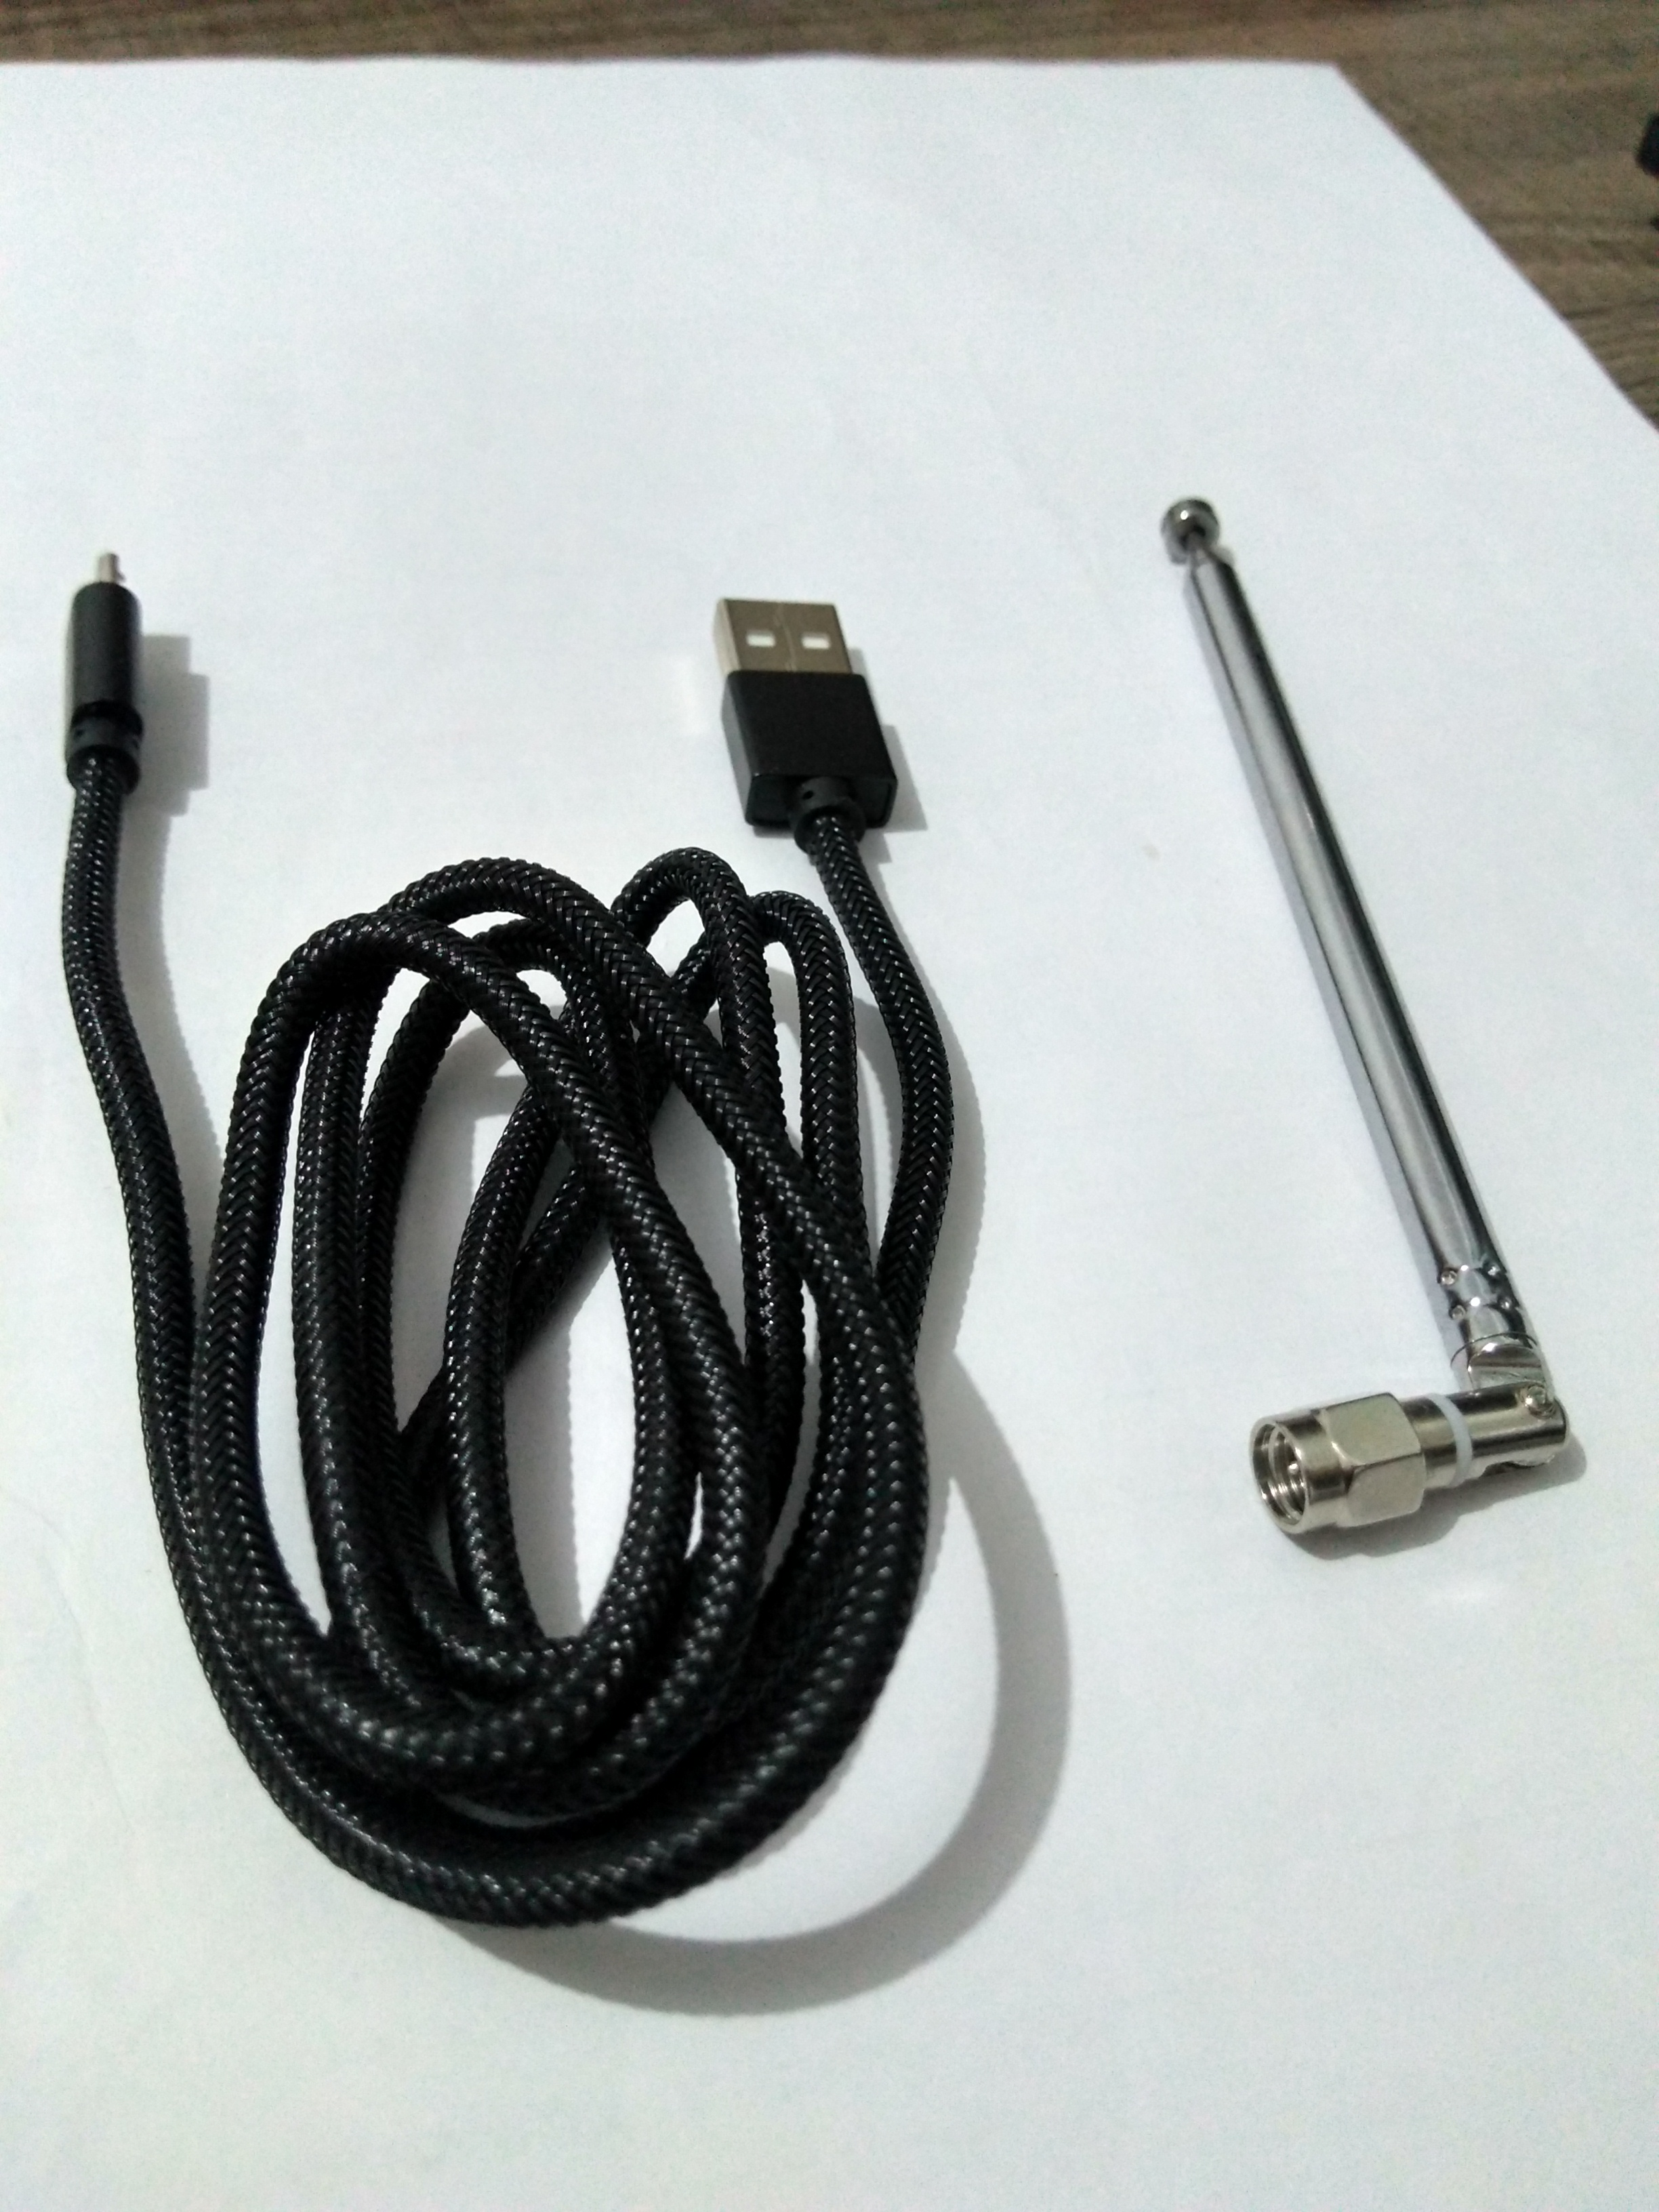
\includegraphics[width=\linewidth]{figures/hackrf/hack_rf_cabo_usb_antena_linear.jpg}
    \caption{Cabo USB e antena telescópica.}
    \label{fig:hack_rf_cabo_usb_antena_linear}
  \end{subfigure}
  \hspace{0.5cm}
  \begin{subfigure}[b]{0.45\linewidth}
    \centering
    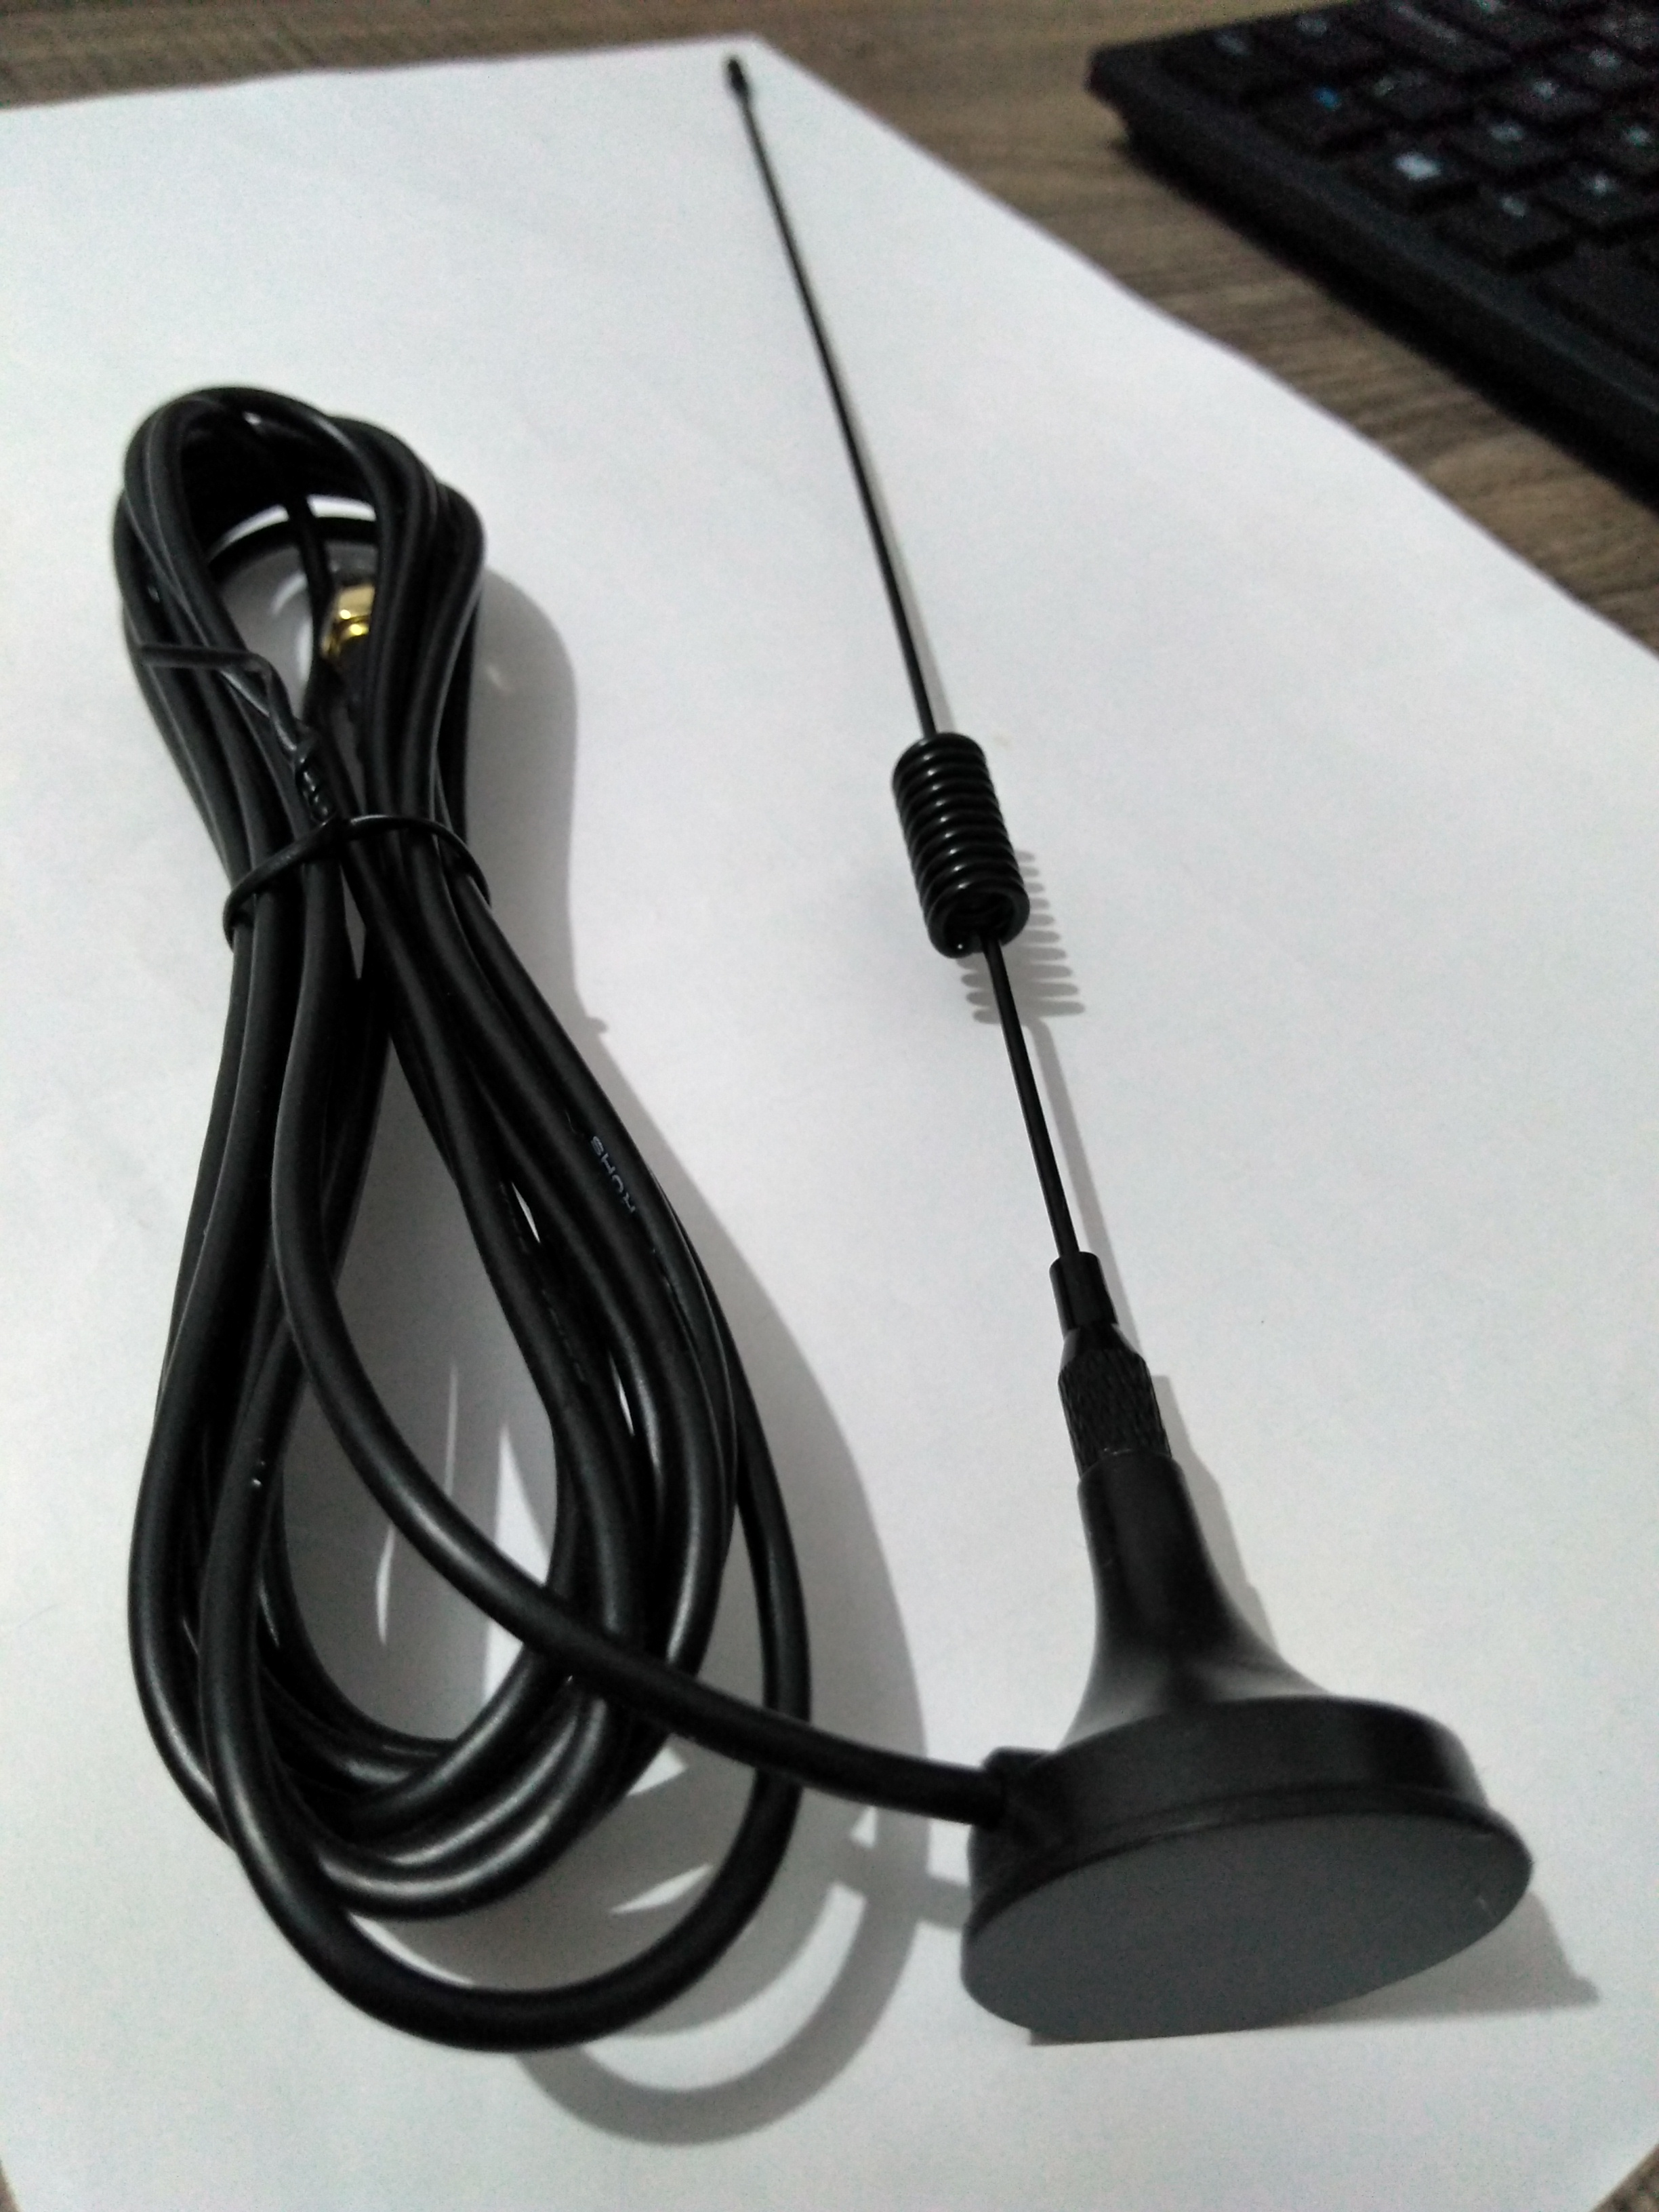
\includegraphics[width=\linewidth]{figures/hackrf/hack_rf_antena_helicoidal.jpg}
    \caption{Antena Omnidirecional.}
    \label{fig:hack_rf_antena_helicoidal}
  \end{subfigure}
  \quad
  \begin{subfigure}[b]{0.45\linewidth}
    \centering
    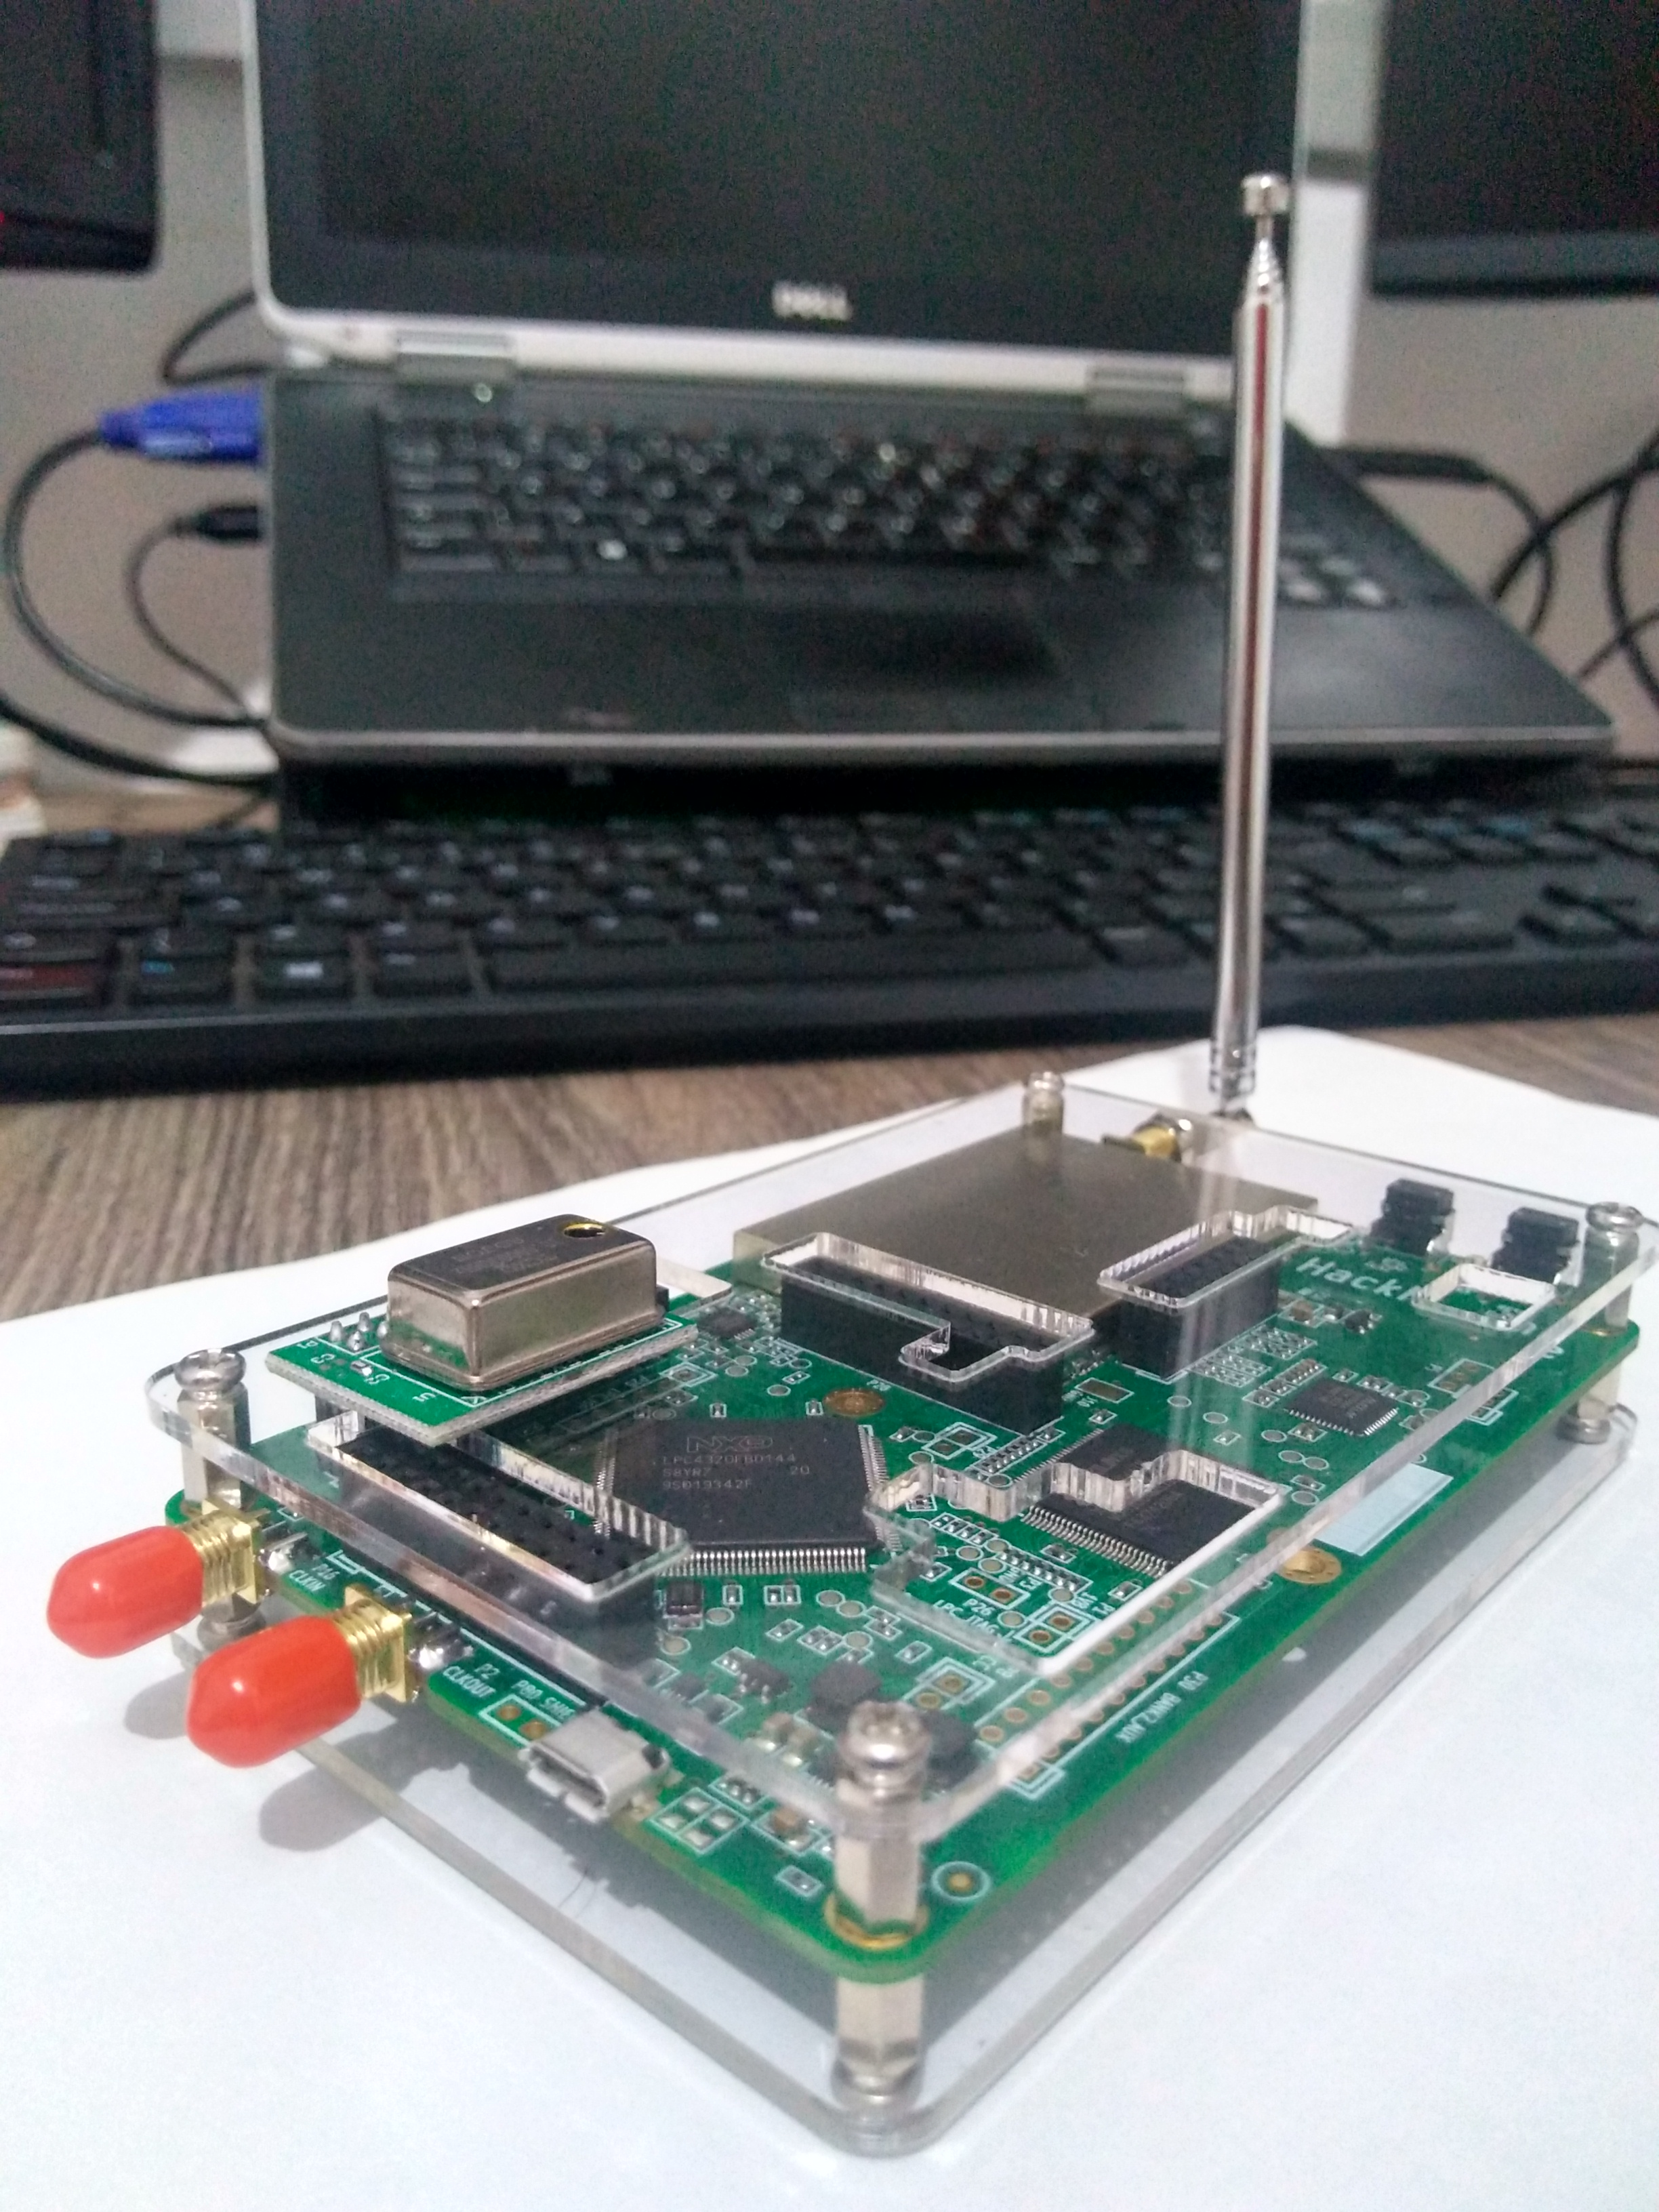
\includegraphics[width=\linewidth]{figures/hackrf/hack_rf.jpg}
    \caption{HackRF com TCXO.}
    \label{fig:hack_rf}
  \end{subfigure}
  \hspace{0.5cm}
  \begin{subfigure}[b]{0.45\linewidth}
    \centering
    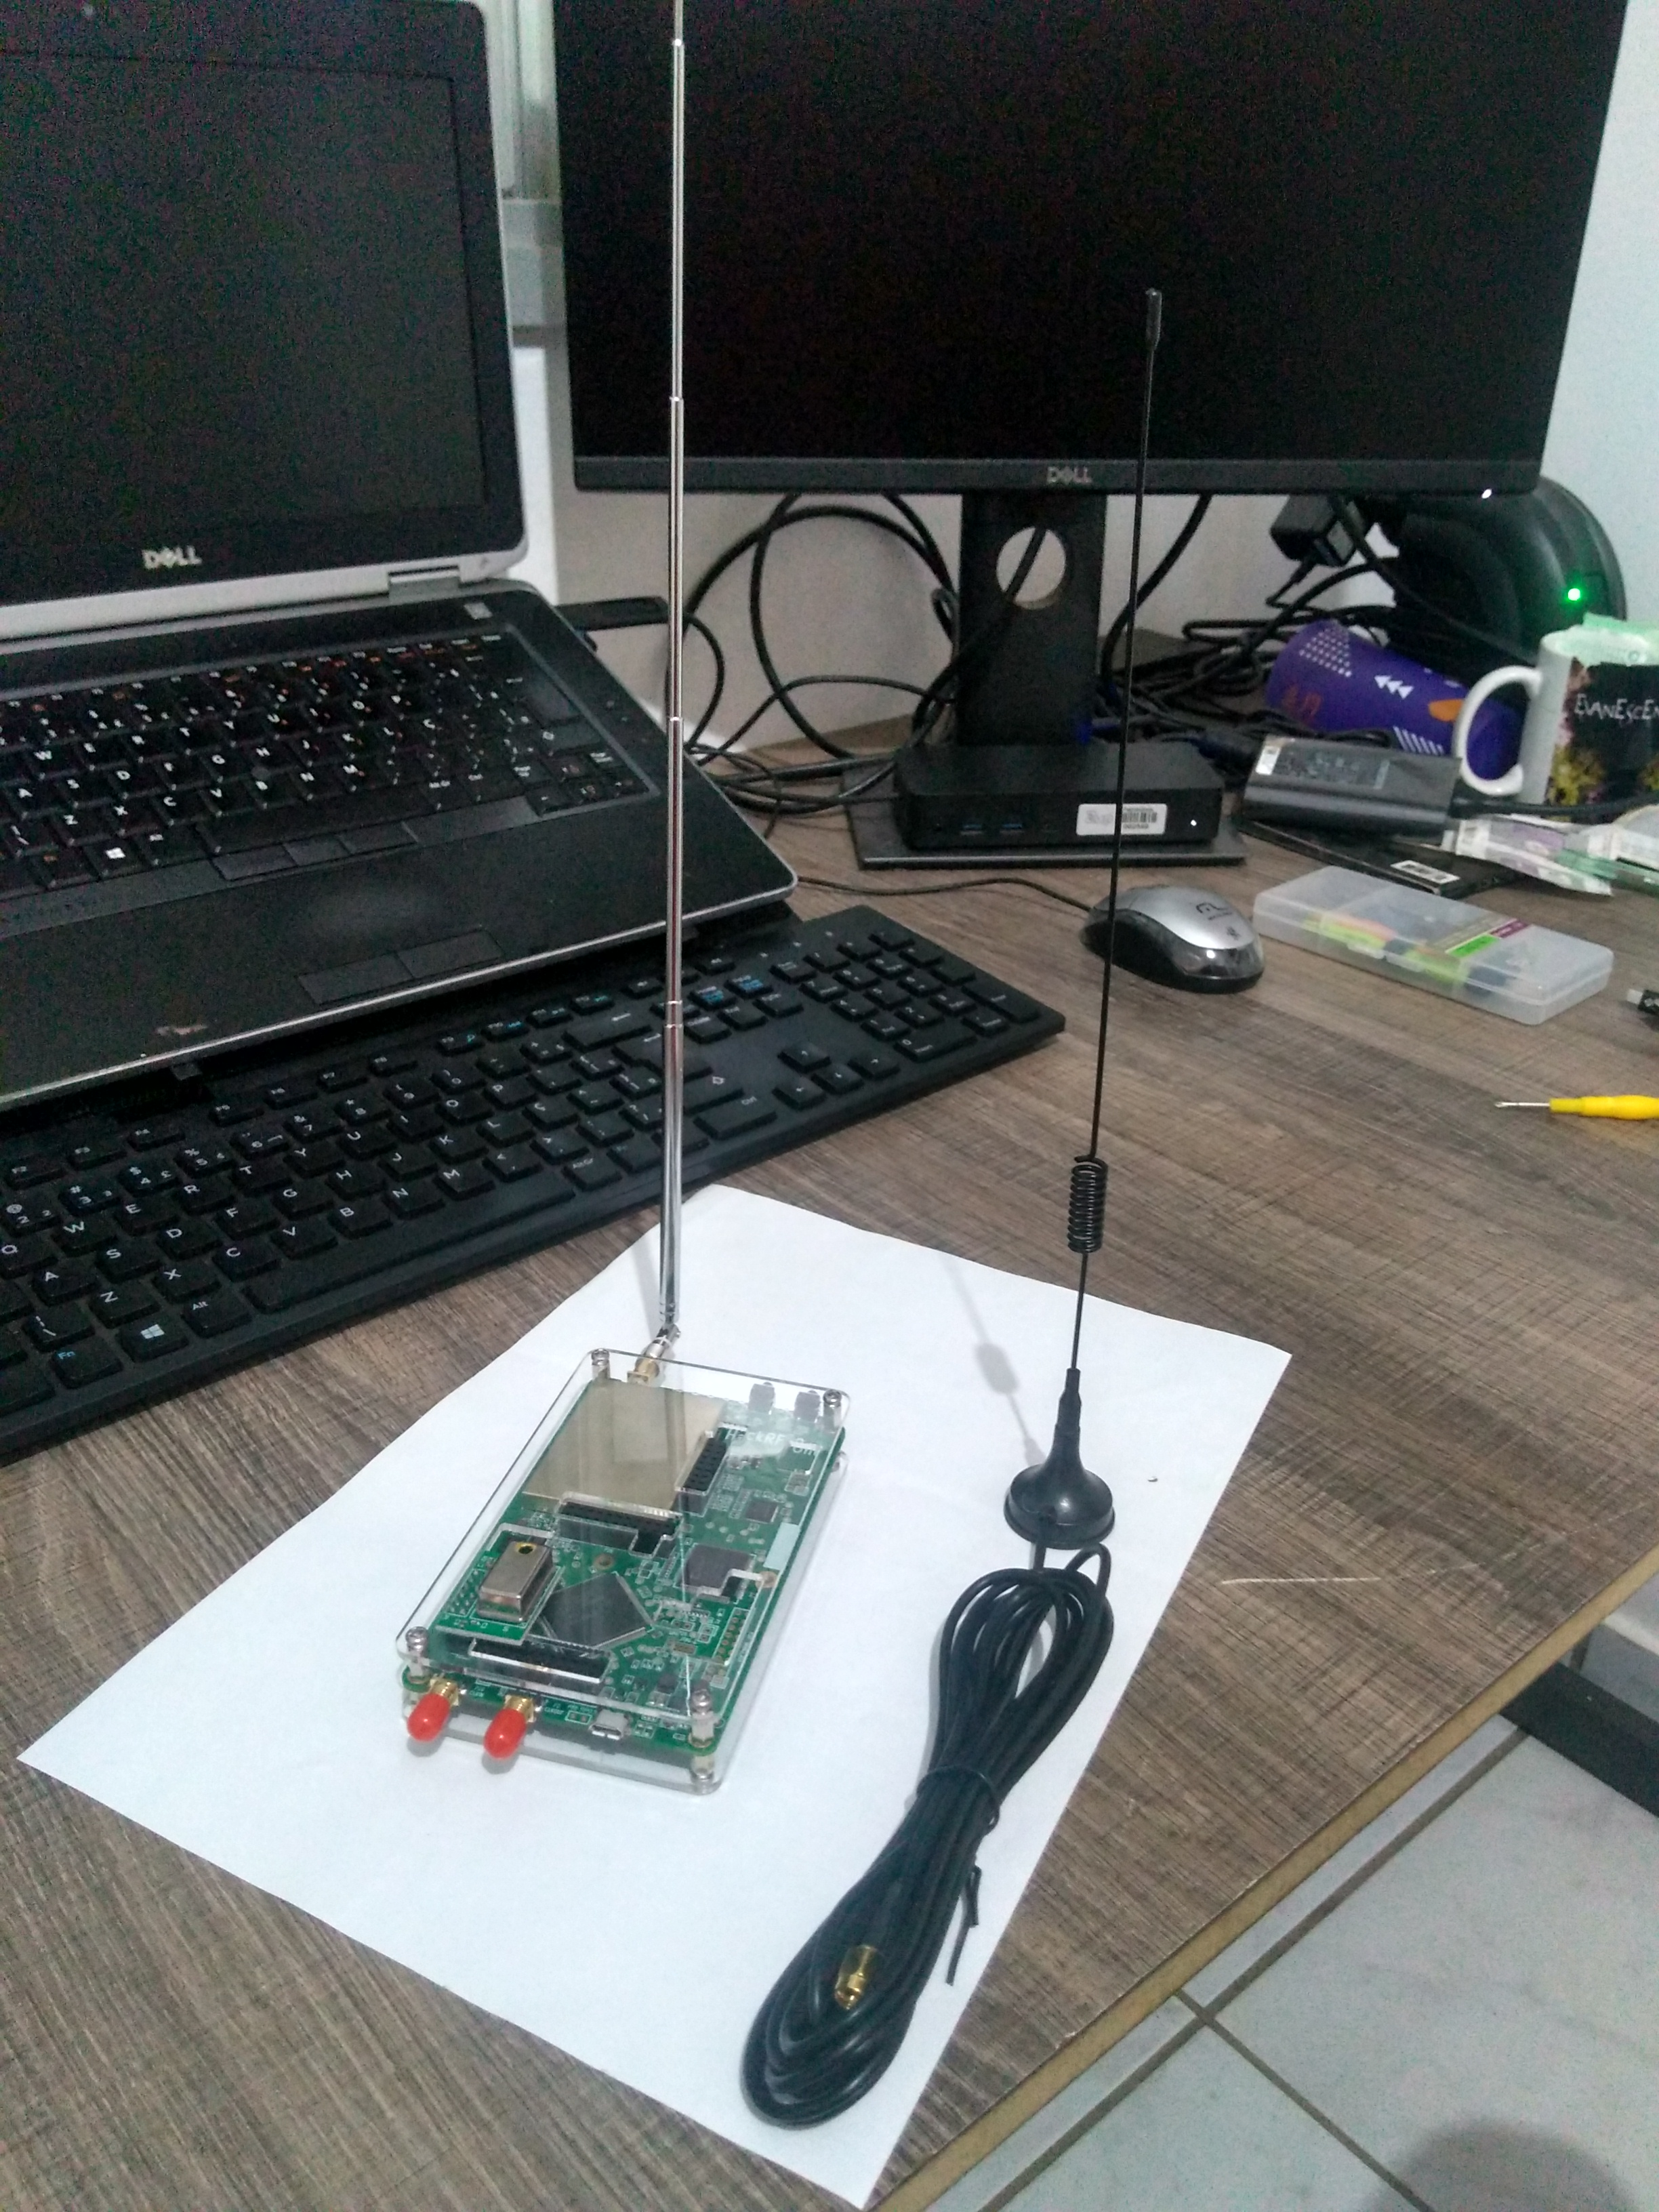
\includegraphics[width=\linewidth]{figures/hackrf/hack_rf_kit.jpg}
    \caption{Kit completo.}
    \label{fig:hack_rf_kit}
  \end{subfigure}
  \caption{\textit{Kit} de desenvolvimento de aplicações de rádio definido por software.}
  \label{fig:hack_rf_hdk}
\end{figure}

\chapter{Software}

O conceito e as boas práticas relacionadas ao desenvolvimento de \textit{software} evoluiu bastante desde os primórdios da computação e algo que sempre esteve
em pauta é o problema de incompatibilidade de ambientes de desenvolvimento, o que acabou dando origem ao jargão: “na minha máquina funciona”.
Configurar o ambiente de desenvolvimento e depois ter incompatibilidade de versão de alguma biblioteca ou então não ter a facilidade de replicar o ambiente
que foi utilizado durante o desenvolvimento é um grande problema enfrentado por engenheiros e/ou programadores, principalmente os que estão em início de carreira.
Nesta parte deste trabalho será demonstrada a criação de um ambiente para desenvolvimento de aplicações de rádio definido por \textit{software} utilizando
o \textbf{GNURadio} instalado em um \textit{container} \textbf{Docker}.
Os conceitos de \textit{container}'s e do \textit{Docker} com certeza já são amplamente abordados na atualidade e então, apenas alguns pontos relacionados ao tema
serão tratados aqui.

\section*{GNURadio}

O GNURadio é um SDK (\textit{software development kit}) de um projeto \textit{OpenSource} criado com o intuito de auxiliar no desenvolvimento de aplicações de
rádio definido por \textit{software} inicialmente publicado no ano de 2001 como um pacote oficial GNU. Este \textit{software} pode ser utilizado tanto por \textit{hobbystas}, como
também em meio acadêmico ou para suprir necessidades do mercado no que tange comunicações sem fio ou qualquer tipo de sistema de rádio digital do mundo real.
O GNURadio está sob uma licença pública geral — GNU GPLv3 — da \textit{Free Software Foundation} (FSF).

Por ser um projeto de \textit{software} agnóstico ao \textit{hardware} das plataformas de desenvolvimento (SDR — \textit{Software-defined Radio}), o GNURadio é idealizado
para trabalhar apenas com dados digitalizados e a partir disso executar todo um processamento digital de sinais (DSP — \textit{Digital Signal Processing})
definido por aplicações escritas para receber ou enviar dados de sistemas de \textit{streaming} digital programaticamente, utilizando a linguagem de programação
Python — que é considerado mais fácil — ou C++ — para escrita de códigos de desempenho crítico — além de também ser possível através de uma interface gráfica de
usuário (\textbf{GNURadio Companion} — GRC) por diagramas de blocos.

\newpage
\section*{Docker}

O \textit{Docker} é uma unidade padrão de \textit{software} da empresa \textit{Docker} Inc., que fornece uma camada de abstração e automação em containers, ou seja, grupos isolados de
processos do \textit{kernel} Linux sendo executados e compartilhando os recursos de um mesmo \textit{host}. Um bom entendimento sobre os \textit{namespaces} do  sistema operacional
Linux (\textbf{mnt}, \textbf{pid}, \textbf{net}, \textbf{ipc}, \textbf{uts}, \textbf{user} e \textbf{cgroups}) pode ajudar na compreensão de quais soluções os
\textit{containers} podem oferecer.

Um questionamento bastante pertinente que pode vir à tona neste momento é: Seria mesmo necessário utilizar \textit{container}'s para criação
do ambiente de desenvolvimento, sendo que o próprio GNURadio já é distribuído oficialmente em pacotes compatíveis com os principais sistemas
operacionais encontrados no mercado? Com o decorrer do próximo capítulo o porquê se tornará mais claro e por agora a ideia principal é de
que quanto mais isolado possível for o ambiente de desenvolvimento, mais fácil será para testar hipóteses, criar diferentes soluções e tornar
possível que elas sejam reproduzidas com facilidade independentemente da plataforma de \textit{hardware}.

Muitas ferramentas que podem ser úteis para engenheiros e desenvolvedores de \textit{software} para gerenciar ou solucionar problemas podem não estar
incluídas no sistema \textit{host} de suas máquinas por padrão e a melhor maneira de adicionar ferramentas a um \textit{host} seria
incluindo-as em um \textit{container} possibilitando que o \textit{host} seja o mais "enxuto" possível.

Os \textit{container}'s são projetados para manter suas próprias visualizações contidas de \textit{namespaces} e têm acesso limitado aos \textit{hosts} nos quais
são executados. Por padrão, os \textit{container}'s têm uma tabela de processos, interfaces de rede, sistemas de arquivos e recursos IPC
(\textit{Inter-Process Communication}) separados do \textit{host}.
Muitos recursos de segurança, como por exemplo o SELinux (\textit{Security-Enhanced Linux}), são colocados em \textit{container}'s para controlar o acesso ao sistema \textit{host} e outros
\textit{container}'s. Embora os \textit{container}'s possam usar recursos do \textit{host}, os comandos executados a partir de um \textit{container} têm uma capacidade muito
limitada de interagir diretamente com o \textit{host}.

Alguns \textit{container}'s, entretanto, têm como objetivo acessar, monitorar e, possivelmente, alterar recursos no sistema \textit{host}
diretamente \cite{RHEL-container:2020}. Eles são chamados de \textit{container}'s super privilegiados (SPC - \textit{Super Privileged Container}). Um desenvolvedor
pode \textit{subir} um SPC em um \textit{host}, solucionar um problema e removê-lo quando não for mais necessário para liberar recursos.

No próximo capítulo é mostrado como utilizar dos \textit{container}'s super privilegiados para a criação do ambiente de
desenvolvimento de aplicações de \textit{software} e como os recursos de um sistema \textit{host} são acessados a partir desse SPC.

\section*{Criação do ambiente de desenvolvimento}

Primeiramente é necessário ter a CLI (\textit{command line interface}) do \textbf{docker engine} instalada (na máquina \textit{host}) e tal procedimento de
instalação se torna extremamente simples bastando seguir o passo-a-passo fornecido pela \href{https://docs.docker.com/engine/install/}{documentação oficial}
do \textit{Docker} \cite{Docker:2020}.
Esta CLI está disponível para várias distribuições Linux na versão \textit{Server} e também para Windows e Mac na versão \textit{Desktop}. Neste trabalho será
demonstrado o procedimento de instalação do \textbf{docker engine} em uma distribuição Linux, de forma que este procedimento é semelhante para demais distribuições
e arquiteturas.

\subsection*{Instalação do \textit{Docker Engine}}

O \textit{Docker} fornece pacotes prontos (\textbf{.deb} e \textbf{.rpm}) para instalação dessa CLI em distribuições Linux como \textit{CentOS}, \textit{Debian},
\textit{Fedora}, \textit{Raspbian}, \textit{Ubuntu} e derivadas (\textit{LMDE}, \textit{BunsenLabs Linux}, \textit{Kali Linux}, \textit{Kubuntu}, \textit{Lubuntu}
e \textit{Xubuntu}, por exemplo) para arquiteturas \textbf{x86\_64}/\textbf{amd64}, \textbf{ARM} (\textit{Advanced RISC Machine}) e \textbf{ARM64}/\textbf{AARCH64}.
Outra opção de instalação seria utilizando os binários pré-compilados que são fornecidos no site do \textit{Docker} e essa forma
faz bastante sentido quando o sistema operacional utilizado não fizer parte de algum dentre todos os suportados
pelo \textit{Docker}.

Antes de iniciar o procedimento de instalação é necessário verificar se o sistema operacional do \textit{host} utilizado está instalado em uma versão de hardware
de arquitetura 64-bit (\textbf{x86\_64} ou \textbf{amd64}, \textbf{armhf} e \textbf{arm64}/\textbf{aarch64}) e não possui instalações de versões antigas
do \textit{software} (\textbf{docker}, \textbf{docker.io}, ou \textbf{docker-engine}) e, caso hajam, é necessário removê-las. No sistema
operacional Ubuntu basta utilizar o gerenciador de pacotes \textbf{apt}/\textbf{apt-get} para fazê-lo, conforme é exemplificado a seguir:

\begin{adjustbox}{max width=\linewidth}
  \begin{lstlisting}[language=bash]
  $ sudo apt-get remove docker-engine \
    docker docker.io containerd runc
  \end{lstlisting}
\end{adjustbox}

\subsubsection*{Instalação utilizando o repositório ofical}

Utilizar o gerenciador de pacotes presente na distribuição Linux facilita o processo de instalação e remoção de \textit{software} do sistema operacional e esta intalação será feita
utilizando o pacote fornecido no repositório oficial do \textit{Docker}. O primeiro
passo é atualizar a lista de pacotes através do comando \textbf{apt-get update} e instalar algumas dependências que permitem que o gerenciador de pacotes (\textbf{apt}) use um repositório sobre HTTPS.
Os comandos são exemplificados como segue:

\newpage
\begin{adjustbox}{max width=\linewidth}
  \begin{lstlisting}[language=bash]

  $ sudo apt-get update

  $ sudo apt-get install \
    apt-transport-https \
    ca-certificates \
    curl \
    gnupg-agent \
    software-properties-common
  \end{lstlisting}
\end{adjustbox}


Após isso é necessário adicionar a chave GPG (\textit{GNU Privacy Guard}) oficial do\textit{Docker} através do comando:

\begin{adjustbox}{max width=\linewidth}
  \begin{lstlisting}[language=bash]
  $ curl -fsSL https://download.docker.com/linux/ubuntu/gpg \
    | sudo apt-key add -
  \end{lstlisting}
\end{adjustbox}

Para verificar se o sistema já possui a chave com o \textit{fingerprint} \textit{Docker} (no momento em que este texto foi escrito,
era \textbf{9DC8 5822 9FC7 DD38 854A E2D8 8D81 803C 0EBF CD88}), o usuário deve pesquisar os últimos 8 caracteres desse \textit{fingerprint}. Neste caso, basta utilizar o comando:

\begin{adjustbox}{max width=\linewidth}
  \begin{lstlisting}[language=bash]
    $ sudo apt-key fingerprint 0EBFCD88
    \end{lstlisting}
\end{adjustbox}

E o retorno do terminal ficará:

\begin{adjustbox}{max width=\linewidth}
  \begin{lstlisting}[language=bash]
  pub   rsa4096 2017-02-22 [SCEA]
  9DC8 5822 9FC7 DD38 854A  E2D8 8D81 803C 0EBF CD88
  uid  [unknown] Docker Release (CE deb) <docker@docker.com>
  sub   rsa4096 2017-02-22 [S]
\end{lstlisting}
\end{adjustbox}

Feito isso, o próximo passo será configurar que o repositório mais estável ("\textit{stable}") do \textit{Docker} seja indexado ao gerenciador de
pactotes do sistema, o \textbf{apt}:

\begin{adjustbox}{max width=\linewidth}
  \begin{lstlisting}[language=bash]
  $ sudo add-apt-repository \
  "deb [arch=amd64] https://download.docker.com/linux/ubuntu \
  $(lsb_release -cs) \
  stable"
\end{lstlisting}
\end{adjustbox}


Finalmente, as versões mais recentes do \textbf{containerd} e do \textit{Engine} do \textit{Docker} podem ser instaladas após atualizar os índices do
gerenciador de pacotes \textbf{apt}.

\begin{adjustbox}{max width=\linewidth}
  \begin{lstlisting}[language=bash]
  $ sudo apt-get update
  $ sudo apt-get install docker-ce \
    docker-ce-cli containerd.io
\end{lstlisting}
\end{adjustbox}

Para verificar se a instalação foi bem-sucedida, basta executar o comando de testes a seguir que é o "\textit{hello-world}" do \textit{Docker}. Se tudo ocorrer bem,
o terminal responderá com uma saída semelhante ao que é mostrado na Fig. \ref{fig:docker-hello-world}.

\begin{adjustbox}{max width=\linewidth}
  \begin{lstlisting}[language=bash]
  $ sudo docker run hello-world
\end{lstlisting}
\end{adjustbox}

\begin{figure}[!htb]
  \centering
  \caption{Teste de verificação de instalação do \textit{Docker Engine}.}
  \includegraphics[width = \linewidth]{figures/docker-hello-world.png}
  Fonte: Elaborado pelo autor.
  \label{fig:docker-hello-world}
\end{figure}

Neste ponto, o \textit{Docker} encontra-se devidamente instalado no sistema operacional e o usuário pode optar por executar alguns comandos de pós-instalação
para, por exemplo, possibilitar a execução do \textit{Docker} sem a necessidade de ter privilégios de usuário \textit{root}, iniciar o serviço \textit{Docker} na inicialização do
sistema operacional, usar uma \textit{engine} de armazenamento diferente da que vem como padrão de instalação (\textit{overlay2}) dentre outras coisas descritas
na seção de \href{https://docs.docker.com/engine/install/linux-postinstall/}{pós-instalação} da documentação oficial \cite{Docker:post-installation-2020}.

\subsection*{Criação do container}

Com o \textit{Docker} instalado, para inciar o procedimento de criação do \textit{container} do ambiente de desenvolvimento é preciso executar o comando \textbf{xhost +}
para fornecer acesso ao servidor gráfico do \textit{host} a aplicações “externas” ao \textit{host} (também conhecido como sessão \textbf{X} ou a tela do computador),
afinal um dos objetivos é utilizar a interface gráfica do \textit{GNURadio Companion} que estará instalado dentro do \textit{container}.

Agora, executando o seguinte comando será criado um \textit{container} a partir de uma imagem base da distribuição \textit{Ubuntu}. A Fig.
\ref{fig:docker-run-gnuradio} exemplifica o uso do comando e as saídas retornadas pelo terminal e é dentro do \textit{container}
criado que será feita a instalação do GNURadio.

\begin{adjustbox}{max width=\linewidth}
  \begin{lstlisting}[language=bash]
$  docker run -i -t --privileged \
    --ipc=host --net=host --pid=host -e HOST=/host \
    -e DISPLAY=$DISPLAY \
    -e DCONF_PROFILE=/etc/dconf/profile/ \
    -e XDG_DATA_HOME=/config/xdg/data \
    -e XDG_CONFIG_HOME=/config/xdg/config \
    -e XDG_CACHE_HOME=/config/xdg/cache \
    -e XDG_RUNTIME_DIR=/tmp/runtime-root \
    -e DBUS_SESSION_BUS_ADDRESS="$DBUS_SESSION_BUS_ADDRESS" \
    -e DEBIAN_FRONTEND="noninteractive" \
    -e IMAGE=jeffcandido/gnuradio \
    -v /run:/run -v /var/log:/var/log\
    -v /etc/localtime:/etc/localtime -v /:/host \
    -v /etc/dconf/profile/:/etc/dconf/profile/ \
    -v /tmp/runtime-root/:/tmp/runtime-root/ \
    -v /tmp/.X11-unix/:/tmp/.X11-unix \
    -v /dev/usb:/dev/usb \
    -v /dev/snd:/dev/snd \
    -v /home/jefferson/gnuradio:/home/jefferson/gnuradio \
    --name gnuradio \
    ubuntu:20.04
  \end{lstlisting}
\end{adjustbox}


\begin{figure}[!htb]
  \centering
  \caption{Criação do \textit{container} de desenvolvimento a partir de uma imagem Ubuntu.}
  \includegraphics[width = \linewidth]{figures/docker-run-gnuradio.png}
  Fonte: Elaborado pelo autor.
  \label{fig:docker-run-gnuradio}
\end{figure}

Para melhorar o entendimento, essa linha vai ser dividida e explicada por partes. O comando \textbf{docker run} primeiro cria uma camada de \textit{container}
gravável sobre a imagem especificada (Ubuntu) e, em seguida, o inicia usando o comando especificado. Ou seja, \textbf{docker run} é equivalente a utilizar
\textbf{docker container create} e depois \textbf{docker container start}. Um \textit{container} interrompido pode ser reiniciado com todas as suas alterações anteriores
intactas usando \textbf{docker start}. Agora, sobre as \textit{flags} passadas:

\begin{itemize}
  \item[$-$] \textbf{i} (\textbf{interactive}): manter o \textbf{STDIN} (\textit{standard input} — fluxo de entrada padrão) aberto, mesmo se não estiver conectado;
  \item[$-$] \textbf{t} (\textbf{tty}): alocar um pseudo-\textbf{TTY} (\textit{TeleTYpewriter} — simplesmente um terminal ao qual o usuário está conectado);
  \item[$-$] \textbf{privileged}: dar privilégios estendidos a este \textit{container} (desativa a separação de segurança entre o \textit{host} e o
        \textit{container}, o que significa que um processo executado como \textit{root} dentro do \textit{container} tem o mesmo acesso ao \textit{host}
        que ele poderia também ter se fosse executado de fora do \textit{container}.);
  \item[$-$] \textbf{e} (\textbf{env}): definir variáveis de ambiente;
  \item[$-$] \textbf{v} (\textbf{volume}): vincular a montagem de um volume dentro \textit{container};
  \item[$-$] \textbf{name}: o nome que se dará ao \textit{container} criado.
  \item[$-$] As \textit{flags} \textbf{--ipc=host}, \textbf{--net=host} e \textbf{--pid=host} desligam os \textit{namespaces} \textbf{ipc},
        \textbf{net} e \textbf{pid} dentro do \textit{container}. Isso significa que os processos dentro do \textit{container} veem a mesma rede e
        tabela de processos, bem como compartilham quaisquer IPCs \cite{Rusling-IPC:1999} com os processos do \textit{host}.
\end{itemize}

Indo um pouco mais a fundo, tem-se a configuração de algumas variáveis de ambiente e a definição dos pontos de montagem e vinculação de alguns
\textit{volumes} ao \textit{host}. Em tese, estas variáveis de ambiente foram configuradas porque foram observadas algumas necessidades durante o
desenvolvimento deste trabalho, tais quais:

\begin{itemize}
  \item[$-$] \textbf{HOST=/host}: definir uma variável que possa ser usada dentro do \textit{container} para acessar
        arquivos e diretórios a partir da raiz do \textit{filesystem} do \textit{host};
  \item[$-$] \textbf{DISPLAY=\$DISPLAY}: definir uma variável que identifique onde serão exibidos recursos pelo servidor gráfico \textbf{X};
  \item[$-$] \textbf{DCONF\_PROFILE=/etc/dconf/profile/}: definir a variável relacionada a um sistema de armazenamento das
        preferências de usuário \cite{GNOME-dconf-overview:2020};
  \item[$-$] \textbf{XDG\_DATA\_HOME=/config/xdg/data}: definir qual será o único diretório base relativo ao qual os arquivos
        de dados específicos do usuário devem ser gravados \cite{freedesktop-XDG:2020};
  \item[$-$] \textbf{XDG\_CONFIG\_HOME=/config/xdg/config}: definir qual será o único diretório base relativo ao qual os arquivos
        de configuração específicos do usuário devem ser gravados \cite{freedesktop-XDG:2020};
  \item[$-$] \textbf{XDG\_CACHE\_HOME=/config/xdg/cache}: definir qual será o único diretório base relativo ao qual os dados não
        essenciais específicos do usuário (em cache) devem ser gravados \cite{freedesktop-XDG:2020};
  \item[$-$] \textbf{XDG\_RUNTIME\_DIR=/tmp/runtime-root}: definir qual será o único diretório base relativo ao qual os arquivos de
        tempo de execução específicos do usuário e outros objetos de arquivo devem ser colocados;
  \item[$-$] \textbf{DBUS\_SESSION\_BUS\_ADDRESS=}

        \textbf{"\$DBUS\_SESSION\_BUS\_ADDRESS"}: possibilitar a inicialização de uma sessão de barramento usando o utilitário D-Bus \cite{freedesktop-DBUS:2020};
  \item[$-$] \textbf{DEBIAN\_FRONTEND="noninteractive"}: definir variável para silenciar os \textit{prompt}'s de configuração do \textit{container} \cite{Debian:non-interactive};
  \item[$-$] \textbf{IMAGE=jeffcandido/gnuradio}: definir a variável para identificar o nome da imagem.
\end{itemize}

Com relação aos \textit{volumes} que foram montados, seguem suas definições:

\begin{itemize}
  \item[$-$] \textbf{/run}:\textbf{/run}: montar o diretório \textbf{/run} do host no diretório \textbf{/run} dentro do \textit{container}. Isso permite que os processos dentro do
        \textit{container} falem com o serviço \textbf{dbus} do \textit{host} e falem diretamente com o serviço \textbf{systemd};

  \item[$-$] \textbf{/var/log}:\textbf{/var/log}: permitir que comandos sejam executados dentro do \textit{container} para ler e gravar arquivos de log no diretório
        \textbf{/var/log} do \textit{host};

  \item[$-$] \textbf{/etc/localtime}:\textbf{/etc/localtime}: fazer com que o fuso horário do sistema \textit{host} seja usado
        tambem no \textit{container};

  \item[$-$] \textbf{/}:\textbf{/host}: montar a raiz da árvore de diretórios do \textit{host} (mais conhecida como \textbf{/}) no  ponto
        de montagem \textbf{/host} para permitir que processos dentro do \textit{container} consigam modificar facilmente o conteúdo no \textit{host};

  \item[$-$] \textbf{/etc/dconf/profile/}:\textbf{/etc/dconf/profile/}: vincular o sistema de armazenamento de preferências do usuário ao mesmo do \textit{host} \cite{RHEL-dconf-profile:2020};

  \item[$-$] \textbf{/tmp/runtime-root/}:\textbf{/tmp/runtime-root/}: montar e vincular o diretório base relativo aos arquivos de
        tempo de execução específicos do usuário;

  \item[$-$] \textbf{/tmp/.X11-unix/}:\textbf{/tmp/.X11-unix/}: montar um volume para o \textit{unix socket} X11 (servidor gráfico);

  \item[$-$] \textbf{/dev/usb}:\textbf{/dev/usb}: vincular o volume que possibilita a utilização de recursos da porta USB do \textit{host};

  \item[$-$] \textbf{/dev/snd}:\textbf{/dev/snd}: vincular o volume que possibilita a utilização de recursos de áudio do \textit{host};

  \item[$-$] \textbf{/home/jefferson/gnuradio}:\textbf{/home/jefferson/gnuradio}: montar um diretório que será utilizado no desenvolvimento
        deste trabalho e que poderá ser acessado tanto pelo \textit{host} como pelo \textit{container}.
\end{itemize}

Resumindo, foi utilizada uma linha de comando para criar um \textit{container}, o qual foi nomeado \textbf{gnuradio}, a partir de uma imagem base (Ubuntu) com
privilégios para acessar recursos da máquina (o \textit{host}), onde mais precisamente será possível utilizar os recursos de áudio, da porta USB e da
interface visual com uma vinculação de volumes montados no \textit{container} a partir da máquina \textit{host}.

Algo importante a se notar na Fig. \ref{fig:docker-run-gnuradio} é que depois da criação do \textit{container} o terminal “mudou” do usuário \textbf{jefferson} para \textbf{root}
e manteve o \textit{hostname}. Isso ocorre porque a partir desse momento o que aparece na tela é o terminal visto de "dentro"
do \textbf{container}, ou seja com o usuário \textbf{root} em um \textit{container} que está enxergando o mesmo \textit{namespace} \textbf{net} que o
sistema \textit{host}.

Em outro terminal é possível obter mais informações como, por exemplo, quais \textit{container}'s estão sendo executados no momento ou inspecionar algum
\textit{container} específico em busca de maiores detalhes, como é mostrado na Fig. \ref{fig:docker-inspect}.

\begin{figure}[!htb]
  \centering
  \caption{Detalhamento de informações sobre \textit{container}’s \textit{Docker}.}
  \includegraphics[width = \linewidth]{figures/docker-inspect.png}
  Fonte: Elaborado pelo autor.
  \label{fig:docker-inspect}
\end{figure}

\newpage
\subsection*{Instalação do GNURadio}

Até o momento apenas foi feito o provisionamento de um \textit{container} \textit{Docker} executando uma imagem Ubuntu e então o GNURadio será instalado utilizando
o gerenciador de pacotes \textbf{apt} disponível na distribuição Ubuntu deste \textit{container}. É recomendável atualizar a lista dos repositórios e verificar
as depedências para esta instalação bastando executar os seguintes comandos no terminal do \textit{container} criado:

\begin{adjustbox}{max width=\linewidth}
  \begin{lstlisting}[language=bash]
  $ apt-get update && apt-get upgrade
  $ apt-get install gir1.2-gtk-3.0 libx11-dev
  $ apt-get install gnuradio
\end{lstlisting}
\end{adjustbox}

A partir desse ponto, o GNURadio estará instalado no \textit{container} \textit{Docker} e é possível verificar a versão, o local de instalação e os
componentes já habilitados através dos seguintes comandos que foram exemplificados na Fig. \ref{fig:gnuradio-config-info}:

\begin{adjustbox}{max width=\linewidth}
  \begin{lstlisting}[language=bash]
  $ gnuradio-config-info --version
  $ gnuradio-config-info --prefix
  $ gnuradio-config-info --enabled-components
\end{lstlisting}
\end{adjustbox}

\begin{figure}[!htb]
  \centering
  \caption{Conferência de versão, \textit{path} e componentes habilitados do GNURadio.}
  \includegraphics[width = \linewidth]{figures/gnuradio-config-info.png}
  Fonte: Elaborado pelo autor.
  \label{fig:gnuradio-config-info}
\end{figure}

Conforme ilustrado na Fig. \ref{fig:gnuradio-companion}, após todos os procedimentos descritos neste capítulo, o GNURadio na versão \textbf{3.8.1.0} estará
disponível para o desenvolvimento de aplicações de rádio definido por \textit{software} e de processamento digital de sinais utilizando as bibliotecas
que foram instaladas no \textit{container} ou utilizando a GUI — \textit{Graphical User Interface}, interface gráfica de usuário —
através do comando \textbf{gnuradio-companion} (GRC).

\begin{figure}[!htb]
  \centering
  \caption{\textit{GUI} do \textit{GNURadio Companion}.}
  \includegraphics[width = \linewidth]{figures/gnuradio-companion.png}
  Fonte: Elaborado pelo autor.
  \label{fig:gnuradio-companion}
\end{figure}

\subsection*{Criação da imagem \textit{Docker}}

O \textit{container} criado na seção anterior pode ser disponibilizado para outros desenvolvedores por meio da criação de uma imagem
base. A imagem base deve receber uma \textit{tag}, que normalmente está ligada à sua versão e por fim esta imagem pode ser
"empurrada" para um repositório de imagens \textit{Docker}. Neste caso foi utilizado o \textit{DockerHub} que é um repositório
de imagens \textit{Docker} hospedado e fornecido pela própria empresa \textit{Docker} Inc. Qualquer empresa pode hospedar, manter
e disponibilizar um repositório de imagens \textit{Docker} por meio da implantação de um \textit{Docker Registry} próprio.

Na Fig. \ref{fig:docker-gnuradio_base_image}, ao executar o comando \textbf{docker images} apenas a imagem \textbf{ubuntu}
foi listada, pois ainda não foi criada uma imagem do container \textbf{gnuradio}, o qual pode ser conferido com o comando
\textbf{docker ps -a}. Utilizando o commando \textbf{docker commit} referenciando para o container \textbf{gnuradio}, uma imagem
\textit{Docker} é criada localmente, onde as \textit{flags} utilizadas, \textbf{-a} e \textbf{-m}, são uma descrição
sobre o autor e uma breve mensagem sobre a imagem criada, respectivamente.

\begin{figure}[!htb]
  \centering
  \caption{Fazendo o \textit{commit} da imagem base GNURadio.}
  \includegraphics[width = \linewidth]{figures/docker-gnuradio_base_image.png}
  Fonte: Elaborado pelo autor.
  \label{fig:docker-gnuradio_base_image}
\end{figure}

Após o \textit{commit} da imagem, ao executar o comando \textbf{docker images} novamente, observa-se que a imagem foi criada com
um \textbf{IMAGE ID} igual a \textbf{1c66799cf780} faltando apenas que seja associada a um repositório e que tenha uma \textit{tag} de versionamento.
Como exemplo foi criada a \textit{tag} para a imagem e associada a um repositório público através do comando \textbf{docker tag 1c66799cf780 jeffcandido/gnuradio}.
Ao executar \textbf{docker images} novamente, a imagem do \textit{container} contendo a instalação do GNURadio na versão 3.8.1.0
está pronta para ser levada ao repositório de imagens \textit{Docker} e se tornar acessível a outros desenvolvedores. Para
fazer esse procedimento, foi necessário criar uma conta (gratuita) no \textit{DockerHub} e fazer o login via linha de comando e por fim
executar o \textit{push} da imagem para levá-la até o repositório remoto, como é demonstrado nos passos executados na Fig. \ref{fig:docker-push_image}.

\begin{figure}[!htb]
  \centering
  \caption{Submetendo a imagem base ao repositório remoto.}
  \includegraphics[width = \linewidth]{figures/docker-push_image.png}
  Fonte: Elaborado pelo autor.
  \label{fig:docker-push_image}
\end{figure}

A imagem que foi criada e submetida ao repositório remoto agora pode ser visualizada pela interface \textit{web} do \textit{DockerHub} e qualquer usuário
conectado à \textit{Internet} poderá buscar e utilizar essa imagem.

\begin{figure}[!htb]
  \centering
  \caption{Interface \textit{web} do \textit{DockerHub} com a imagem \textit{Docker} criada.}
  \includegraphics[width = \linewidth]{figures/dockerhub-general.png}
  Fonte: Elaborado pelo autor.
  \label{fig:dockerhub-general}
\end{figure}

Algumas otimizações poderiam ser feitas com relação ao processo de criação do \textit{container} e geração de imagem \textit{Docker}, como por exemplo a criação
de arquivos para composição do \textit{container} (\textit{Dockerfile}, \textit{docker-compose.yaml} e \textit{.dockerignore}), porém isto
não adicionaria vigor e relevância ao propósito deste trabalho de forma que tais otimizações podem ser realizadas em trabalhos futuros nessa mesma
área de estudo.

\subsection*{Instalação do firmware do \textit{HackRF One}}

A forma de instalação do \textit{firmware} e utilitários do \textit{HackRF One} recomendada pelo fabricante é utilizando o gerenciador de pacotes disponibilizado pelo
sistema operacional que neste caso é o \textit{apt}, porém o \textit{software} a ser executado na máquina \textit{host} também pode ser compilado através do código-fonte \cite{HACKRF-build-host-software}. Foi necessário instalar o \textit{HackRF One} como um periférico de rádio definido por \textit{software} com o
apoio dos pacotes \textbf{hackrf} (utilitários), \textbf{libhackrf-dev} (biblioteca para desenvolvimento), \textbf{libhackrf0} (biblioteca para tempo de execução),
\textbf{gr-osmosdr} (Blocos do GNURadio do projeto OsmoSDR) e \textbf{gqrx-sdr} (receptor de rádio definido por \textit{software}).

\begin{adjustbox}{max width=\linewidth}
  \begin{lstlisting}[language=bash]
  $ apt-get install hackrf libhackrf-dev libhackrf0 gqrx-sdr gr-osmosdr
\end{lstlisting}
\end{adjustbox}

Para atualizar o firmware do \textit{HackRF One} basta baixar a versão desejada diretamente do repositório oficial do projeto e seguir os passos
definidos na documentação \cite{HACKRF-updating-firmware} que nada mais é que escrever o executável na memória \textit{flash} da placa (\textit{hackrf\_spiflash -w hackrf\_one\_usb.bin}).
Realizado este procedimento, é possível verificar que o dispositivo foi instalado corretamente utilizando os comandos \textbf{hackrf\_info} e \textbf{hackrf\_transfer} \cite{HACKRF-tools}, conforme mostra a Fig. \ref{fig:hackrf_info}.

\begin{figure}[!htb]
  \centering
  \caption{Verificação de versão do \textit{firmware} do \textit{HackRF One}.}
  \includegraphics[width = \linewidth]{figures/hackrf/hackrf_info_version_transfer}
  Fonte: Elaborado pelo autor.
  \label{fig:hackrf_info}
\end{figure}
% ----------------------------------------------------------
% Parte de desenvolvimento
% ----------------------------------------------------------
\part{Desenvolvimento}

\chapter{Criação de \textit{flowgraph}'s no GNURadio}

Neste ponto o objetivo é demonstrar fluxos simples de processamento digital de sinais utilizando os GNURadio e nada mais justo que iniciar esta parte
do trabalho desmonstrando \textit{flowgraph}'s de operações matemáticas básicas aplicadas a sinais digitais assim como utilizações convenientes do processamento de sinais.

Para o primeiro \textit{flowgraph} foram posicionadas duas fontes de sinal de frequências distintas (2 kHz e 20 kHz) e suas saídas foram agregadas em um bloco de soma de sinais. Após isso,
para que as formas de onda dos sinais possam ser visualizadas, foram adicionados os blocos \textit{QT GUI} para apresentação dos sinais nos domínios do tempo
(\textit{Time Sink}) e da frequência (\textit{Frequency Sink}). O bloco \textit{Throtle} normalmente é utilizado na saída de blocos que não são de origem
diretamente de \textit{hardware}, com o objetivo de limitar a taxa na qual esse bloco cria as amostras.

\begin{figure}[!htb]
  \centering
  \begin{subfigure}[b]{0.8\linewidth}
    \centering
    \caption{\textit{Flowgraph} da soma de dois sinais.}
    \includegraphics[width = \linewidth, trim = 0.1cm 10cm 20cm 4cm, clip=true]{figures/signals/01_sum_flowgraph}
    \label{fig:gnuradio_sum_flowgraph}
  \end{subfigure}

  \begin{subfigure}[b]{0.8\linewidth}
    \centering
    \caption{Gráficos da soma de dois sinais no GNURadio.}
    \includegraphics[width = \linewidth]{figures/signals/sum}
    \label{fig:gnuradio_sum}
  \end{subfigure}
  \caption{Processamento da soma de dois sinais utilizando o GNURadio.}
  \label{fig:gnuradio_signals_sum}
\end{figure}

Ao executar o código gerado pelo \textit{flowgraph} da Fig. \ref{fig:gnuradio_sum_flowgraph}, a interface do \textit{GNURadio-companion} constrói na Fig. \ref{fig:gnuradio_sum} os gráficos
relacionados à soma dos sinais, tanto no domínio do tempo como no domínio dam frequência. De forma semelhante, na Fig. \ref{fig:gnuradio_product_flowgraph} está o \textit{flowgraph} para
operação do produto de dois sinais que podem ser visualizados pela interface gráfica na Fig. \ref{fig:gnuradio_product}.

\begin{figure}[!htb]
  \centering
  \begin{subfigure}[b]{0.8\linewidth}
    \centering
    \caption{\textit{Flowgraph} do produto de dois sinais.}
    \includegraphics[width = \linewidth, trim = 0.1cm 10cm 20cm 4cm, clip=true]{figures/signals/02_product_flowgraph}
    \label{fig:gnuradio_product_flowgraph}
  \end{subfigure}

  \begin{subfigure}[b]{0.8\linewidth}
    \centering
    \caption{Gráficos do produto de dois sinais no GNURadio.}
    \includegraphics[width = \linewidth]{figures/signals/product}
    \label{fig:gnuradio_product}
  \end{subfigure}
  \caption{Processamento do produto de dois sinais utilizando o GNURadio.}
  \label{fig:gnuradio_signals_product}
\end{figure}

Foram criados também dois \textit{flowgraph}'s, apresentados nas Figs. \ref{fig:gnuradio_delay_flowgraph} e \ref{fig:gnuradio_hysteresis_flowgraph}, que têm objetivos bastante
conhecidos por engenheiros em eletrônica e telecomunicações, que são o entendimento sobre a defasagem entre sinais (Figs. \ref{fig:gnuradio_delay_flowgraph} e \ref{fig:gnuradio_delay})
e também o conceito de histerése (Figs. \ref{fig:gnuradio_hysteresis_flowgraph}
\ref{fig:gnuradio_hysteresis}) utilizado na comparação de sinais, principalmente aqueles sobre o efeito de ruído.

\begin{figure}[!htb]
  \centering
  \begin{subfigure}[b]{\linewidth}
    \centering
    \caption{\textit{Flowgraph} para geração de dois sinais defasados no tempo.}
    \includegraphics[width = \linewidth]{figures/signals/03_delay_flowgraph}
    \label{fig:gnuradio_delay_flowgraph}
  \end{subfigure}

  \begin{subfigure}[b]{\linewidth}
    \centering
    \caption{Sinais defasados no domínio do tempo.}
    \includegraphics[width = \linewidth]{figures/signals/delay}
    \label{fig:gnuradio_delay}
  \end{subfigure}
  \caption{Variação de fase entre sinais utilizando o GNURadio.}
  \label{fig:gnuradio_signals_delay}
\end{figure}

\begin{figure}[!htb]
  \centering
  \begin{subfigure}[b]{\linewidth}
    \centering
    \caption{\textit{Flowgraph} para simulação de um comparador de sinais com histerése.}
    \includegraphics[width = \linewidth]{figures/signals/04_hysteresis_flowgraph}
    \label{fig:gnuradio_hysteresis_flowgraph}
  \end{subfigure}

  \begin{subfigure}[b]{\linewidth}
    \centering
    \caption{Comparação de sinais com histerése.}
    \includegraphics[width = \linewidth]{figures/signals/hysteresis}
    \label{fig:gnuradio_hysteresis}
  \end{subfigure}
  \caption{Comparação com histerése de sinais utilizando o GNURadio.}
  \label{fig:gnuradio_signals}
\end{figure}

\chapter{O \textit{Hello-World} do GNURadio}

Neste capítulo será reproduzido o \textit{flowgraph} que é considerado o "\textit{hello-world}" do GNURadio com o hardware do SDR: o receptor de rádio FM. Trata-se de um \textit{flowgraph}
bastante simples, pois todos os blocos necessários já foram disponibilizados anteriormente nos procedimentos de instalação do GNURadio e do \textit{firmware} do \textit{HackRF One}.

O sinal de rádio FM recebido pelo \textit{hardware} do \textit{HackRF One} sintonizado na frequência portadora de 106.5 MHz (um canal de rádio local com programação ativa na cidade
de Uberlândia, Minas Gerais) passa por um filtro passa-baixas (LPF - \textit{Low-Pass Filter}) de ganho unitário com resposta finita ao impulso unitário
(FIR - \textit{Finite Impulse Response}), frequência de corte de 75 kHz, largura de banda de transição de 25 kHz (com janela de Hamming) e fator de redução da frequência de amostragem
(decimação) de 20:1. Em cascata o sinal é convoluído com um filtro FIR polifásico de reamostragem racional (Rational Resampler) com fator da razão entre as constantes de interpolação
e decimação do sinal igual a $\frac{12}{5}$ e, por fim, é demodulado e novamente decimado para que possa ser consumido pelo bloco \textit{Audio Sink} (repodução do áudio nos
alto-falantes do computador) e que seu espectro seja apresentado utilizando um bloco coletor gráfico para exibição de sinais em frequência (via FFT - \textit{Fast Fourier Transform}),
o \textit{QT GUI Frequency Sink}.

\begin{figure}[!htb]
  \centering
  \caption{\textit{Flowgraph} para simulação de um receptor de rádio FM.}
  \includegraphics[width = \linewidth]{figures/signals/fm_receiver_flowgraph}
  \label{fig:gnuradio_fm_receiver_flowgraph}
  Fonte: Elaborado pelo autor.
  \label{fig:gnuradio_signals_fm_receiver_flowgraph}
\end{figure}

\begin{figure}[!htb]
  \centering
  \caption{\textit{FFT plot} extraída durante simulação do receptor FM.}
  \includegraphics[width = \linewidth]{figures/signals/demodulated_fm_signal}
  \label{fig:gnuradio_demodulated_fm_signal}
  Fonte: Elaborado pelo autor.
  \label{fig:gnuradio_signals_demodulated_fm_signal}
\end{figure}

% AUDIO SINK

% Permite que um sinal seja reproduzido por meio de seus alto-falantes ou outro dispositivo de áudio

% Parâmetros
% Taxa de amostragem

% Para definir a taxa de amostragem de áudio, clique no menu suspenso para ver as taxas populares. Nota: nem todas as taxas de amostragem serão suportadas por seu hardware. Para aplicações típicas, isso deve ser definido para 48 kHz.
% Nome do dispositivo
% Deixe o nome do dispositivo em branco para escolher o dispositivo de áudio padrão. A seleção de um nome de dispositivo específico depende do sistema operacional.

% Linux

% No Linux, as opções típicas incluem:

% hw: 0,0
% plughw: 0,0
% pulso

% Para usuários ALSA com problemas de áudio, siga este procedimento:

% em uma janela de terminal, digite:

% aplay -L

% encontre a entrada como:

% hw: CARD = Genérico, DEV = 0
% HD-Audio genérico, ALC662 rev3 analógico
% Dispositivo de hardware direto sem nenhuma conversão

% da lista que corresponde ao seu dispositivo. Para usar um monitor HDMI com alto-falantes, encontre uma entrada apropriada com "HDMI" nele.

% use a primeira linha dessa entrada (por exemplo, "hw: CARD = Generic, DEV = 0") como o nome do dispositivo. A menos que o nome contenha espaços, as aspas são opcionais.

% OK para bloquear

% Ativado por padrão, que deve ser usado quando este coletor não for regulado por nenhum outro bloco.
% Num Inputs
% O coletor de áudio pode ter várias entradas dependendo do seu hardware. Por exemplo, defina as entradas como 2 para estéreo ou 1 para mono.


% http://sdr.osmocom.org/trac/wiki/GrOsmoSDR


% https://osmocom.org/projects/gr-osmosdr/wiki/GrOsmoSDR
% osmocom\_siggen\_nogui -a hackrf -f 100e6 --sine
% osmocom\_siggen\_nogui -a hackrf -f 100e6 --sweep -x 2M -y 1 -c34
% osmocom\_siggen\_nogui -a hackrf -f 100e6 --sweep -x 2e6 -y 10 -v


\chapter{Criando blocos customizados}

% OutOfTreeModules

% Estendendo o GNU Radio com funcionalidades e blocos próprios

% Este artigo se baseia muito no original (mas muito desatualizado) "Como escrever um bloco?" escrito por Eric Blossom.

% O que é um módulo fora da árvore?

% Um módulo fora da árvore é um componente do GNU Radio que não reside na árvore de origem do GNU Radio. Normalmente, se você deseja estender o GNU Radio com suas próprias funções e
% blocos, esse módulo é o que você cria (ou seja, você não costuma adicionar coisas à árvore de fontes do GNU Radio real a menos que esteja planejando enviá-lo aos desenvolvedores
% para integração upstream). Isso permite que você mesmo mantenha o código e tenha funcionalidades adicionais junto com o código principal.

% Muitos projetos OOT estão hospedados na CGRAN - a Comprehensive GNU Radio Archive Network. Os projetos CGRAN estão todos disponíveis através de nossa ferramenta PyBOMBS. Na verdade,
% quando você adiciona seu projeto ao repositório de receitas PyBOMBS, ele atualiza automaticamente o site CGRAN.

% Ferramentas e recursos à minha disposição

% Existem algumas ferramentas, scripts e documentos que estão disponíveis como programas de terceiros ou como parte do GNU Radio.

% gr\_modtool - O canivete suíço da edição de módulos

% Ao desenvolver um módulo, há muito trabalho chato e monótono envolvido: código clichê, edição de makefile, etc. gr\_modtool é um script que visa ajudar com todas essas coisas,
% editando automaticamente makefiles, usando modelos e fazendo o máximo de trabalho possível para o desenvolvedor, de forma que você possa ir direto para a codificação DSP.

% Observe que gr\_modtool faz muitas suposições sobre a aparência do código. Quanto mais o seu módulo for personalizado e tiver mudanças específicas, menos útil será o gr\_modtool,
% mas é provavelmente o melhor lugar para começar com qualquer novo módulo ou bloco.

% gr\_modtool agora está disponível na árvore de fontes do GNU Radio e é instalado por padrão.
% Recursos para desenvolvedores na wiki

% O mais importante é definitivamente o guia de codificação de blocos. Embora seja escrito para a árvore principal do GNU Radio, também deve ser aplicado a todos os módulos.
% Especificamente, dê uma olhada nas convenções de nomenclatura!

% section*{Block coding guide}

% \textbf{Terminologia}

% Block A unidade de processamento funcional com entradas e saídas
% Port Uma única entrada ou saída de um bloco
% Source de dados Fonte A
% Sink Um consumidor de dados
% Connection Um fluxo de dados da porta de saída para a porta de entrada
% Flow graph Uma coleção de blocos e conexões
% Item Uma unidade de dados. Ex: amostra de banda base, vetor fft, matriz ...
% Stream Um fluxo contínuo de itens consecutivos
% IO signature Uma descrição das portas de entrada e saída de blocos

% \textbf{Estrutura de Código}

% \textbf{Public Header Files}

% Os arquivos de cabeçalho públicos são definidos em include / foo e são instalados em \$ prefix / include / foo.

% As funções acessoras (set / get) que devem ser exportadas são definidas como funções virtuais puras neste cabeçalho.

% Um esqueleto de um arquivo de cabeçalho público comum se parece com:

% \begin{adjustbox}{max width=\linewidth}
%   \begin{lstlisting}[language=C++]
%     #ifndef INCLUDED_FOO_BAR_H
%     #define INCLUDED_FOO_BAR_H
    
%     #include <foo/api.h>
%     #include <gr_sync_block.h>
    
%     namespace gr {
%       namespace foo {
        
%       class FOO_API bar : virtual public gr_sync_block
%       {
%       public:
%         // gr::foo::bar::sptr
%         typedef boost::shared_ptr sptr;
        
%         /*!
%         * \class bar
%         * \brief A brief description of what foo::bar does
%         *
%         * \ingroup _blk
%         *
%         * A more detailed description of the block.
%         *
%         * \param var explanation of argument var.
%         */

%         static sptr make(dtype var);
        
%         virtual void set_var(dtype var) = 0;
%         virtual dtype var() = 0;
%       };
%     } /* namespace foo */
%   } /* namespace gr */
  
%   #endif /* INCLUDED_FOO_BAR_H */
%   \end{lstlisting}
% \end{adjustbox}

% \textbf{Implementation Header File}

% Os arquivos de cabeçalho de implementação privada são definidos em lib e não são instalados. Normalmente definimos esses arquivos para usar o mesmo nome que o arquivo público
% e classe com um sufixo \_impl para indicar que este é o arquivo de implementação para a classe.

% Em alguns casos, esse arquivo pode ser específico para uma implementação muito particular e várias implementações podem estar disponíveis para um determinado bloco, mas com a
% mesma API pública. Um bom exemplo é o uso da biblioteca FFTW para implementar os blocos fft\_filter. Esta é apenas uma das muitas maneiras possíveis de implementar um FFT e,
% portanto, a implementação foi nomeada fft\_filter\_ccc\_fftw. Outra biblioteca que implementa um FFT específico para uma plataforma ou propósito pode então ser encaixada como uma
% nova implementação como fft\_filter\_ccc\_myfft.

% % Todas as variáveis ​​de membro são declaradas privadas e usam o prefixo d\_. Tanto quanto possível, todas as variáveis ​​devem ter uma função set e get. A função set se parece
% com void set\_var (dtype var), e a função get se parece com dtype var(). Nem sempre faz sentido ter um conjunto ou obter uma determinada variável, mas todos os esforços devem
% ser feitos para acomodá-lo.

% Os comentários do Doxygen que serão incluídos no manual são definidos no arquivo de cabeçalho público. Não há necessidade de marcação Doxygen nos arquivos privados, mas é claro,
% qualquer comentário ou documentação que faça sentido sempre deve ser usado.

% Um esqueleto de um arquivo de cabeçalho privado comum se parece com:

% \begin{adjustbox}{max width=\linewidth}
%   \begin{lstlisting}[language=C++]
%     #ifndef INCLUDED_FOO_BAR_IMPL_H
%     #define INCLUDED_FOO_BAR_IMPL_H

%     #include <foo/bar.h>
    
%     namespace gr {
%       namespace foo {
        
%       class FOO_API bar_impl : public bar
%       {
%       private:
%         dtype d_var;
%       public:
%         bar_impl(dtype var);
        
%         ~bar_impl();
        
%         void set_var(dtype var);
%         dtype var();
        
%         int work(int noutput_items,
%             gr_vector_const_void_star &input_items,
%             gr_vector_void_star &output_items);
%       };
%     } /* namespace foo */
%   } /* namespace gr */
  
%   #endif /* INCLUDED_FOO_BAR_IMPL_H */
%   \end{lstlisting}
% \end{adjustbox}

% \textbf{Implementation Source File}

% O arquivo fonte é lib / bar.cc e implementa o código real para a classe.

% Este arquivo define a função make para a classe pública. Este é um membro da classe, o que significa que podemos, se necessário, fazer coisas interessantes, definir
% funções de múltiplos fatores, etc. Na maioria das vezes, isso simplesmente retorna um sptr para a classe de implementação.

% \begin{adjustbox}{max width=\linewidth}
%   \begin{lstlisting}[language=C++]
%     #ifdef HAVE_CONFIG_H
%     #include "config.h"
%     #endif
    
%     #include "bar_impl.h"
%     #include <gr_io_signature.h>

%     namespace gr {
%       namespace foo {
        
%         bar::sptr bar::make(dtype var)
%         {
%           return gnuradio::get_initial_sptr(new bar_impl(var));
%         }
    
%         bar_impl::bar_impl(dtype var)
%           : gr_sync_block("bar",
%                   gr_make_io_signature(1, 1, sizeof(in_type)),
%                   gr_make_io_signature(1, 1, sizeof(out_type)))
%         {
%           set_var(var);
%         }
    
%         bar_impl::~bar_impl()
%         {
%           // any cleanup code here
%         }
        
%         dtype
%         bar_impl::var()
%         {
%           return d_var;
%         }
    
%         void
%         bar_impl::set_var(dtype var)
%         {
%           d_var = var;
%         }
        
%         int
%         bar_impl::work(int noutput_items,
%                         gr_vector_const_void_star &input_items,
%                         gr_vector_void_star &output_items)
%         {
%           const in_type *in = (const in_type*)input_items[0];
%           out_type *out = (out_type*)output_items[0];
      
%           // Perform work; read from in, write to out.
%           return noutput_items;
%         }
%       } /* namespace foo */
%     } /* namespace gr */
%   \end{lstlisting}
% \end{adjustbox}

% \textbf{SWIG Interface File}

% Devido ao uso do arquivo de cabeçalho público para descrever o que queremos acessível publicamente, podemos simplesmente incluir os cabeçalhos no arquivo de interface
% principal. Portanto, no diretório swig está um único arquivo de interface foo\_swig.i:

% \begin{adjustbox}{max width=\linewidth}
%   \begin{lstlisting}[language=C++]
%     #define FOO_API

%     %include "gnuradio.i" 

%     //load generated python docstrings
%     %include "foo_swig_doc.i" 

%     %{
%       #include "foo/bar.h" 
%     %}

%     %include "foo/bar.h" 

%     GR_SWIG_BLOCK_MAGIC2(foo, bar);
%   \end{lstlisting}
% \end{adjustbox}

% \textbf{Block Structure}

% The \textbf{work} function

% Para implementar o processamento, o usuário deve escrever uma rotina de "trabalho" que lê entradas, processa e escreve saídas.

% Um exemplo de função WORK implementando um somador em cplusplus:

% \begin{adjustbox}{max width=\linewidth}
%   \begin{lstlisting}[language=C++]
%     int work(int noutput_items,
%               gr_vector_const_void_star &input_items,
%               gr_vector_void_star &output_items)
%     {
      
%       //cast buffers
%       const float* in0 = reinterpret_cast<const float*>(input_items[0]);
%       const float* in1 = reinterpret_cast<const float*>(input_items[1]);
%       float* out = reinterpret_cast<float*>(output_items[0]);
  
%       //process data
%       for(size_t i = 0; i < noutput_items; i++) {
%         out[i] = in0[i] + in1[i];
%       }
  
%       //return produced
%       return noutput_items;
%     }
%   \end{lstlisting}
% \end{adjustbox}

% Definições de parâmetros:

% noutput\_items: número total de itens em cada buffer de saída
% input\_items: vetor de buffers de entrada, onde cada elemento corresponde a uma porta de entrada
% output\_items: vetor de buffers de saída, onde cada elemento corresponde a uma porta de saída

% Algumas observações:

% Cada buffer deve ser convertido de um ponteiro void * em um tipo de dados utilizável.
% O número de itens em cada buffer de entrada está implícito em noutput\_items
% Mais informações sobre isso nas seções posteriores
% O número de itens produzidos é retornado, pode ser menor que noutput\_items


% \textbf{IO signatures}

% Ao criar um bloco, o usuário deve comunicar o seguinte ao bloco:

% O número de portas de entrada
% O número de portas de saída
% O tamanho do item de cada porta

% Uma assinatura IO descreve o número de portas que um bloco pode ter e o tamanho de cada item em bytes. Cada bloco tem 2 assinaturas de E/S: uma assinatura de entrada e
% uma assinatura de saída.

% Alguns exemplos de assinaturas em cplusplus

% \begin{adjustbox}{max width=\linewidth}
%   \begin{lstlisting}[language=C++]
%     -- A block with 2 inputs and 1 output --

%     gr_sync_block("my adder", gr_make_io_signature(2, 2, sizeof(float)), gr_make_io_signature(1, 1, sizeof(float)))

%     -- A block with no inputs and 1 output --

%     gr_sync_block("my source", gr_make_io_signature(0, 0, 0), gr_make_io_signature(1, 1, sizeof(float)))

%     -- A block with 2 inputs (float and double) and 1 output --

%     std::vector input_sizes;

%     input_sizes.push_back(sizeof(float));

%     input_sizes.push_back(sizeof(double));

%     gr_sync_block("my block", gr_make_io_signaturev(2, 2, input_sizes), gr_make_io_signature(1, 1, sizeof(float)))
%   \end{lstlisting}
% \end{adjustbox}

% Algumas observações:

% Use gr\_make\_io\_signature para blocos onde todas as portas são homogêneas em tamanho
% Use gr\_make\_io\_signaturev para blocos que têm tamanhos de porta heterogêneos

% Os primeiros dois parâmetros são o número mínimo e máximo de portas, o que permite que os blocos tenham um número selecionável de portas em tempo de execução.

% Tipos de bloco

% Para tirar proveito da estrutura gnuradio, os usuários criarão vários blocos para implementar o processamento de dados desejado. Existem vários tipos de blocos para escolher:

% Blocos síncronos (1: 1)
% Blocos de Decimação (N: 1)
% Blocos de interpolação (1: M)
% Blocos Gerais (N: M)

% Bloco Síncrono

% O bloco de sincronização permite aos usuários escrever blocos que consomem e produzem um número igual de itens por porta. Um bloco de sincronização pode ter qualquer número de entradas ou saídas. Quando um bloco de sincronização tem zero entradas, é chamado de fonte. Quando um bloco de sincronização tem zero saídas, é chamado de dissipador.

% Um exemplo de bloco de sincronização em cplusplus.

% \begin{adjustbox}{max width=\linewidth}
%   \begin{lstlisting}[language=C++]
%     #include <gr_sync_block.h>
    
%     class my_sync_block : public gr_sync_block
%     {
%     public:
%       my_sync_block(...):
%         gr_sync_block("my block",
%                       gr_make_io_signature(1, 1, sizeof(int32_t)),
%                       gr_make_io_signature(1, 1, sizeof(int32_t)))
%       {
%         //constructor stuff
%       }
  
%       int work(int noutput_items,
%                 gr_vector_const_void_star &input_items,
%                 gr_vector_void_star &output_items)
%       {
%         //work stuff...
%         return noutput_items;
%       }
%     };
%   \end{lstlisting}
% \end{adjustbox}

% Algumas observações:

% noutput\_items é o comprimento em itens de todos os buffers de entrada e saída
% uma assinatura de entrada de gr\_make\_io\_signature (0, 0, 0) torna este um bloco de origem
% uma assinatura de saída de gr\_make\_io\_signature (0, 0, 0) torna isso um bloco coletor

% \textbf{Decimation Block}

% O bloco de decimação é outro tipo de bloco de taxa fixa em que o número de itens de entrada é um múltiplo fixo do número de itens de saída.

% Um exemplo de bloco de decimação em cplusplus

% \begin{adjustbox}{max width=\linewidth}
%   \begin{lstlisting}[language=C++]
%     #include <gr_sync_decimator.h>
    
%     class my_decim_block : public gr_sync_decimator
%     {
%     public:
%       my_decim_block(...):
%         gr_sync_decimator("my decim block",
%                       in_sig,
%                       out_sig,
%                       decimation)
%       {
%         //constructor stuff
%       }
  
%       //work function here...
%     };
%   \end{lstlisting}
% \end{adjustbox}

% Algumas observações:

% O construtor gr\_sync\_decimator leva um quarto parâmetro, o fator de decimação. O usuário deve assumir que o número de itens de entrada = itens de saída * decimação

% \textbf{Interpolation Block}

% O bloco de interpolação é outro tipo de bloco de taxa fixa em que o número de itens de saída é um múltiplo fixo do número de itens de entrada.

% Um exemplo de bloco de interpolação em cplus

% \begin{adjustbox}{max width=\linewidth}
%   \begin{lstlisting}[language=C++]
%     #include <gr_sync_interpolator.h>
    
%     class my_interp_block : public gr_sync_interpolator
%     {
%     public:
%       my_interp_block(...):
%         gr_sync_interpolator("my interp block",
%                       in_sig,
%                       out_sig,
%                       decimation)
%       {
%         //constructor stuff
%       }
  
%       //work function here...
%     };
%   \end{lstlisting}
% \end{adjustbox}

% Algumas observações:

% O construtor gr\_sync\_interpolator leva um quarto parâmetro, o fator de interpolação. O usuário deve assumir que o número de itens de entrada = itens de saída / interpolação

% \textbf{Basic Block}

% O bloco básico não fornece relação entre o número de itens de entrada e o número de itens de saída. Todos os outros blocos são apenas simplificações do bloco básico.
% Os usuários devem escolher herdar do bloco básico quando os outros blocos não forem adequados.

% O adicionador revisitado como um bloco básico em cplusplus

% \begin{adjustbox}{max width=\linewidth}
%   \begin{lstlisting}[language=C++]
%     #include <gr_block.h>


%     class my_basic_block : public gr_block

%     {
%     public:

%       my_basic_adder_block(...):
%         gr_block("another adder block",

%                 in_sig,

%                 out_sig)
%       {
%         //constructor stuff
%       }

%       int general_work(int noutput_items,
%                       gr_vector_int &ninput_items,
%                       gr_vector_const_void_star &input_items,
%                       gr_vector_void_star &output_items)
%       {
%         //cast buffers
%         const float* in0 = reinterpret_cast<const float*>(input_items[0]);
%         const float* in1 = reinterpret_cast<const float*>(input_items[1]);
%         float* out = reinterpret_cast<float*>(output_items[0]);

%         //process data
%         for(size_t i = 0; i < noutput_items; i++) {
%           out[i] = in0[i] + in1[i];
%         }

%         //consume the inputs

%         //consume port 0 input
%         this->consume(0, noutput_items);
%         //consume port 1 input
%         this->consume(1, noutput_items);
%         //or shortcut to consume on all inputs
%         //this->consume_each(noutput_items);

%         //return produced
%         return noutput_items;
%       }
%     };
%   \end{lstlisting}
% \end{adjustbox}

% Algumas observações:

% Esta classe sobrecarrega o método general\_work (), não work ()
% O trabalho geral tem um parâmetro: ninput\_items
% ninput\_items é um vetor que descreve o comprimento de cada buffer de entrada
% Antes do retorno, general\_work deve consumir manualmente as entradas usadas
% O número de itens nos buffers de entrada é considerado noutput\_items
% Os usuários podem alterar esse comportamento sobrecarregando o método forecast ()

% \textbf{Other Types of Blocks}

% \textbf{Hierarchical Block}

% Os blocos hierárquicos são blocos compostos por outros blocos. Eles instanciam os outros blocos GNU Radio (ou outros blocos hierárquicos) e os conectam. Um bloco hierárquico possui uma função “conectar” para este propósito.

% Os blocos hierárquicos definem um fluxo de entrada e saída de maneira muito semelhante aos blocos normais. Para conectar a entrada i a um bloco hierárquico, a fonte é (em Python):

% self.connect ((self, <i>), <block>)

% Da mesma forma, para enviar o sinal para fora do bloco no fluxo de saída o:

% self.connect (<block>, (self, <o>))

% Top Block
% O bloco superior é a estrutura de dados principal de um fluxograma GNU Radio. Todos os blocos estão conectados sob este bloco. O bloco superior possui as funções que controlam
% o funcionamento do fluxograma. Geralmente, criamos uma classe que herda de um bloco superior:

% \begin{adjustbox}{max width=\linewidth}
%   \begin{lstlisting}[language=python]
%     class my_topblock(gr.top_block):
%     def __init__(self, ):
%         gr.top_block.__init__(self)
    
%     def main():
%         tb = mytb()
%         tb.run()
%   \end{lstlisting}
% \end{adjustbox}

% O bloco superior tem algumas funções-membro principais:

% start (N): inicia o gráfico de fluxo em execução com N como o máximo de noutput\_items que qualquer bloco pode receber.
% parar (): pára o bloco superior
% wait (): bloqueia até que o bloco superior seja concluído
% executar (N): um início de bloqueio (N) (as chamadas começam e depois esperam)
% lock (): bloqueia o fluxograma para que possamos reconfigurá-lo
% unlock (): desbloqueia e reinicia o fluxograma

% O conceito N nos permite ajustar a latência de um fluxograma. Por padrão, N é grande e os blocos passam grandes pedaços de itens entre si. Isso é projetado para maximizar
% o rendimento e a eficiência. Como grandes blocos de itens incorrem em latência, podemos forçar esses blocos a um tamanho máximo para controlar a latência geral em detrimento
% da eficiência. Um método set\_max\_noutput\_items (N) é definido para um bloco superior para alterar este número, mas ele só tem efeito durante um procedimento de bloqueio / desbloqueio.

% \textbf{Stream Tags}

% Uma tag decora um stream com metadados. Uma tag é associada a um determinado item em um fluxo. Um item pode ter mais de uma tag associada a ele. A associação de um item e tag é
% feita por meio de uma contagem absoluta. Cada item em um fluxo tem uma contagem absoluta. As marcas usam essa contagem para identificar qual item em um fluxo ao qual estão associadas.

% Uma tag tem os seguintes membros:

% deslocamento: a contagem única de itens
% chave: uma chave PMT única para o tipo de conteúdo
% valor: um PMT contendo o conteúdo desta tag
% srcid: um id PMT exclusivo para o produtor da tag (opcional)

% Um PMT é um tipo de dados especial em gnuradio para serializar dados arbitrários. Para saber mais sobre PMTs, consulte mingau / pmt.h

% Reading stream tags

% As tags podem ser lidas na função de trabalho usando get\_tags\_in\_range. Cada porta / fluxo de entrada pode ter tags associadas.

% Exemplo de leitura de tags em cplusplus:

% \begin{adjustbox}{max width=\linewidth}
%   \begin{lstlisting}[language=C++]
%     int work(int noutput_items,
%               gr_vector_const_void_star &input_items,
%               gr_vector_void_star &output_items)
              
%     {
%       std::vector tags;
%       //number of items read on port 0
%       const uint64_t nread = this->nitems_read(0);
%       //assumption for sync block, this can change
%       const size_t ninput_items = noutput_items;
%       //read all tags associated with port 0 for items in this work function
%       this->get_tags_in_range(tags, 0, nread, nread+ninput_items);
%       //work stuff here\dots
%     }
%   \end{lstlisting}
% \end{adjustbox}

% Writing stream tags

% As tags podem ser escritas a partir da função de trabalho usando add\_item\_tag. Cada porta / fluxo de saída pode ter tags associadas.

% Exemplo de gravação de tags em Cplusplus:

% \begin{adjustbox}{max width=\linewidth}
%   \begin{lstlisting}[language=C++]
%     int work(int noutput_items,
%               gr_vector_const_void_star &input_items,
%               gr_vector_void_star &output_items)
%     {
%       const size_t item_index = ? //which output item gets the tag?
%       const uint64_t offset = this->nitems_written(0) + item_index;
%       pmt::pmt_t key = pmt::string_to_symbol("example_key");
%       pmt::pmt_t value = pmt::string_to_symbol("example_value");
  
%       //write at tag to output port 0 with given absolute item offset
%       this->add_item_tag(0, offset, key, value);
  
%       //work stuff here...
%     }
%   \end{lstlisting}
% \end{adjustbox}

% Tips and Tricks

% Esta é a parte do guia onde damos dicas e truques para fazer blocos que funcionam de forma robusta com o planejador.
% Bloqueio de chamadas

% Se uma função de trabalho contém uma chamada de bloqueio, ela deve ser escrita de forma que possa ser interrompida por threads de reforço. Quando o gráfico de fluxo é interrompido,
% todos os threads de trabalho serão interrompidos. A interrupção do thread ocorre quando o usuário chama desbloquear () ou parar () no gráfico de fluxo. Portanto, só é aceitável
% bloquear indefinidamente em uma chamada de thread de impulso, uma variável de suspensão ou condição, ou algo que use essas chamadas de thread de impulso internamente, como
% pop\_msg\_queue (). Se você precisar bloquear um recurso como um descritor de arquivo ou socket, a rotina de trabalho deve sempre chamar a rotina de bloqueio com um tempo limite.
% Quando a operação atinge o tempo limite, a rotina de trabalho deve chamar um ponto de interrupção do thread de reforço ou verificar o thread de reforço interrompido e sair se
% verdadeiro.

% Salvando estado

% % Como as funções de trabalho podem ser interrompidas, as variáveis ​​de estado do bloco podem ser indeterminadas na próxima vez que o gráfico de fluxo for executado. Para tornar os
% blocos robustos contra o estado indeterminado, os usuários devem sobrecarregar as funções start () e stop () dos blocos. A rotina start () é chamada quando o gráfico de fluxo é
% iniciado antes do thread de trabalho () ser gerado. A rotina stop () é chamada quando o gráfico de fluxo é interrompido depois que o thread de trabalho foi unido e encerrado.
% % Os usuários devem garantir que as variáveis ​​de estado do bloco sejam inicializadas com propriedade na rotina start ().

% \textbf{CMake, make, etc.}

% GNU Radio usa CMake como um sistema de construção. Construir um módulo, portanto, requer que você tenha o cmake instalado e qualquer gerenciador de construção de sua preferência
% (na maioria das vezes, é 'make', mas você também pode estar usando Eclipse ou MS Visual Studio).

O objetivo deste capítulo é disponibilizar uma visão geral de como é possível que qualquer um seja também um desenvolvedor de módulos (os quais são chamados de módulos \textit{OOT - Out of Three} \cite{GNURADIO-oot-modules})
de processamento digital de sinais no GNURadio e não apenas usuários da ferramenta \textit{GNURadio-companion}. Para auxiliar no entendimento, será mostrado um passo a passo de como criar
um módulo do GNURadio, adicionar blocos a ele e depois disponibilizar pacotes de instalação que podem ser aproveitados por outros desenvolvedores que estejam direcionados a esse mesmo propósito.

\section*{Módulos \textit{OutOfThree}}

\begin{figure}[!htb]
  \centering
  \caption{Geração de um módulo \textit{OOT} do GNURadio e sua estrutura de arquivos e pastas.}
  \includegraphics[width = \linewidth]{figures/gr_modtool/gr_modtool_newmod_exemplo.png}
  Fonte: Elaborado pelo autor.
  \label{fig:gr_modtool_newmod_exemplo}
\end{figure}

Primeiramente, um módulo fora da árvore (\textit{OOT module}) recebe esse nome por se tratar de um "pedaço" de \textit{software} que pode fazer uso das bibliotecas do GNURadio, mas separado dos
módulos que já foram disponibilizados em uma versão oficial e já se encontram na árvore do GNURadio. Neste módulo o engenheiro pode desenvolver blocos com objetivos específicos sem haver a necessidade
de alterar o que já existe na raiz do projeto do GNURadio, de forma que esse tipo de ramificação permite que o próprio desenvolvedor mantenha o código e disponibilize-o da forma que achar conveniente.

A Fig. \ref{fig:gr_modtool_newmod_exemplo} mostra a execução da ferramenta \textbf{gr\_modtool} para a criação de um módulo de exemplo (chamado de \textit{exemplo}), o qual conterá um
bloco de processamento digital  de sinais que será responsável por simplesmente receber amostras do tipo ponto flutuante e entregar em sua saída o valor da entrada elevado à segunda potência.
Nesta mesma figura é mostrada a estrutura de pastas criada pelo comando \textbf{gr\_modtool}.

Uma simples linha de comando utilizando a ferramenta \textbf{gr\_modtool} cria toda a estrutura de arquivos e pastas de um novo módulo do GNURadio. Os arquivos dos códigos escritos em
\textit{python} devem ir para a pasta \textbf{python/}, os arquivos escritos em C++ devem ser colocados na pasta \textbf{lib/} e os seus arquivos de cabeçalho (\textbf{*.h}) devem ir para a pasta
\textbf{include/}. Também é criada uma pasta relacionada ao \textbf{swig}, que é um \textit{wrapper} (um empacotador) simplificado e gerador de interfaces que cria automaticamente o
código em \textit{python} dos blocos, mesmo que eles tenham sido escritos em C++.

\begin{figure}[!htb]
  \centering
  \caption{Criação dos arquivos de um bloco customizado usando \textbf{gr\_modtool}.}
  \includegraphics[width = \linewidth]{figures/gr_modtool/gr_modtool_add_ao_quadrado.png}
  Fonte: Elaborado pelo autor.
  \label{fig:gr_modtool_add_ao_quadrado}
\end{figure}

Para disponibilizar os blocos via interface gráfica do \textit{GNURadio-companion}, basta adicionar suas descrições na pasta \textbf{grc/} (na versão 3.8 são arquivos \textbf{.yaml} e
antes da versão 3.8 eram arquivos \textbf{.xml}). A pasta \textbf{docs/} contém, intuitivamente, as instruções sobre como as documentações devem ser extraídas dos arquivos C++ e Python
utilizando a bibliotecas \textit{Doxygen} e \textit{Sphinx}. Para compilação do código, o desenvolvedor deve se atentar ao arquivo \textit{CMakeLists.txt} e à pasta \textbf{cmake/} para garantir
as instruções a serem passadas para o programa \textit{Cmake} sobre como encontrar as bibliotecas necessárias e também garantir que o módulo seja compilado corretamente.

O passo seguinte (ilustrado na Fig. \ref{fig:gr_modtool_add_ao_quadrado}) foi criar os arquivos relacionados a um bloco de exemplo, o qual foi nomeado \textit{ao\_quadrado\_ff}, também através de uma simples linha de comando utilizando a ferramenta
\textbf{gr\_modtool}. A nomeação do bloco foi escolhida seguindo uma conveção de nomenclatura dos blocos que consiste na concatenação do nome customizado do bloco com os indicadores de quais são
os tipos de que serão recebidos na entradas e quais serão entregues na saída após serem processados ("\textit{ao\_quadrado\_}" + "\textit{\textbf{f}loat \textbf{f}loat}"). As flags passadas
estão relacionadas ao tipo do bloco (-t \textit{general}, bloco de uso geral) e o tipo de linguagem (-l \textit{cpp}) a ser usada para escrever suas funções.

\begin{figure}[!htb]
  \centering
  \caption{Prática do desenvolvimento guiado por testes.}
  \includegraphics[width = \linewidth]{figures/gr_modtool/qa_ao_quadrado.png}
  Fonte: Elaborado pelo autor.
  \label{fig:qa_ao_quadrado}
\end{figure}

Criar blocos customizados do GNURadio é uma ótima oportunidade para colocar em prática os passos gerais de uma metodologia de desenvolvimento guiada por testes (TDD -
\textit{Test Driven Development}) que são: escrever um teste, compilá-lo e fazê-lo rodar e depois realizar correções para tornar o código correto \cite{KentBeck:TDD-2002}. A Fig.
\ref{fig:qa_ao_quadrado} traz o arquivo \textit{python/qa\_ao\_quadrado\_ff.py} onde foi adicionada a função \textit{test\_001\_ao\_quadrado\_ff} que possui amostras de dados de
entrada e dados que são esperados na saída para realizar comparações com os resultados gerados pelo código escrito.

Com relação aos arquivos do código em C++, basta editar o conteúdo da classe de implementação do bloco (\textit{lib/ao\_quadrado\_ff\_impl.cc}) e seus arquivos de cabeçalho
(\textit{lib/ao\_quadrado\_ff\_impl.h} \textit{include/exemplo/ao\_quadrado\_ff.h}) quando necessário. De forma resumida, na implementação do código em C++ o desenvolvedor terá que descrever
no construtor da classe a "assinatura" das entradas e saídas do bloco, ou seja, quantas entradas de um determinado tipo e quantas saídas, também com a definição de seus tipos, serão reservadas conforme
ilustra a Fig. \ref{fig:ao_quadrado_cc}.
Outro ponto importante é que na função \textit{forecast} deve ser informada a relação entre quantos itens são necessários na entrada para gerar uma quantidade específica de itens na saída.

\begin{figure}[!htb]
  \centering
  \caption{Classe do bloco de processamento digital de sinais customizado.}
  \includegraphics[width = \linewidth]{figures/gr_modtool/ao_quadrado_cc.png}
  Fonte: Elaborado pelo autor.
  \label{fig:ao_quadrado_cc}
\end{figure}

Agora, para tornar o bloco disponível através da interface gráfica do \textit{GNURadio-companion} é necessário gerar o arquivo \textbf{.yaml} que contém as descrições necessárias do bloco e
este procedimento também é realizável utilizando a ferramenta \textit{gr\_modtool}.

\begin{figure}[!htb]
  \centering
  \caption{Geração do arquivo de descrição do bloco na GUI.}
  \includegraphics[width = \linewidth]{figures/gr_modtool/ao_quadrado_make_yaml.png}
  Fonte: Elaborado pelo autor.
  \label{fig:ao_quadrado_make_yaml}
\end{figure}

Para finalizar, é necessário realizar alguns procedimentos para compilar o código, gerar os arquivos binários executáveis e também os pacotes (\textbf{.deb} e \textbf{.rpm}) que tornam
possível a disponibilização do trabalho realizado para outros desenvolvedores através dos gerenciadores de pacotes dos sistemas operacionais. Estes procedimentos são muito importantes,
pois um grande diferencial do engenheiro é ir além da função de programar as aplicações, estando preparado para atuar em todos os passos do processo de criação,
implantação e suporte do \textit{software} que pode ser ou não comercializado.

Para tornar possível a geração de um pacote \textbf{.deb} do bloco customizado, foi necessário adicionar ao final do arquivo \textit{CMakeLists.txt}
que fica na raiz do módulo (\textbf{gr-exemplo}) as três seguintes linhas:

\begin{adjustbox}{max width=\linewidth}
  \begin{lstlisting}[language=C++]
    SET(CPACK_GENERATOR "DEB")
    SET(CPACK_DEBIAN_PACKAGE_MAINTAINER "Jefferson da Silva Candido")
    INCLUDE(CPack)
  \end{lstlisting}
\end{adjustbox}

O procedimento de geração de uma \textit{release} do \textit{software}, quando configurado corretamente, segue um conjunto de passos simples de serem executados, os quais consistem em criar um diretório
dentro da raiz do projeto e dentro dele realizar a construção dos arquivos para produção, a execução dos testes unitários e de integração do código e por fim a instalação.

\begin{adjustbox}{max width=\linewidth}
  \begin{lstlisting}[language=bash]
  $ mkdir build
  $ cd build/
  $ cmake ../
  $ make
  $ make test
  $ make install
  \end{lstlisting}
\end{adjustbox}

\begin{figure}[!htb]
  \centering
  \caption{Geração dos pacotes \textbf{.deb} e \textbf{.rpm}.}
  \includegraphics[width = \linewidth]{figures/gr_modtool/gr_exemplo_build.png}
  Fonte: Elaborado pelo autor.
  \label{fig:gr_exemplo_build}
\end{figure}

\newpage
Os pacotes que podem ser instalados em sistemas compatíveis com as distribuições \textit{Debian} e \textit{CentOS} foram gerados com o auxílio dos programas \textbf{cpack} e \textbf{alien} como mostra a
Fig. \ref{fig:gr_exemplo_build}.

% ----------------------------------------------------------
% Parte de resultados
% ----------------------------------------------------------
\part{Resultados}

% ---
% Capitulo de revisão de literatura
% ---
\chapter{Revisão Literária}

% ---
\section*{Aliquam vestibulum fringilla lorem}

\begin{figure}[!htb]
  \centering
  \caption{Utilização do bloco customizado em um \textit{flowgrpah}.}
  \includegraphics[width = \linewidth]{figures/gr_modtool/exemplo_flowgraph.png}
  Fonte: Elaborado pelo autor.
  \label{fig:exemplo_flowgraph}
\end{figure}
% ---

% \lipsum[1]

% \lipsum[2-3]

% ---
% Finaliza a parte no bookmark do PDF
% para que se inicie o bookmark na raiz
% e adiciona espaço de parte no Sumário
% ---
\phantompart

% ---
% Considerações Finais
% ---
\chapter{Considerações Finais}
% ---

Todos os objetivos previstos para este trabalho foram alcançados e felizmente foi possível trazer em uma abordagem ampla, mesmo que introdutória, alguns conceitos importantes essenciais
no auxílio a engenheiros e desenvolvedores de aplicações de rádio definido por software. Trabalhos futuros a partir deste podem ser realizados de diversas maneiras, como por exemplo:

* utilização do SDR para levantamento da resposta em frequência de dispositivos transmissores;

* Construção de diferentes tipos de moduladores de sinais digitais (BPSK, QPSK, QAM, etc \ldots);

* Criação de transmissores dentro dos padrões do mercado (DVB, ISDB, ATSC, etc \ldots);

* Implementação prática de filtros digitais customizados.


% \lipsum[31-33]

% ----------------------------------------------------------
% ELEMENTOS PÓS-TEXTUAIS
% ----------------------------------------------------------
\postextual

% ----------------------------------------------------------
% Referências bibliográficas
% ----------------------------------------------------------
\bibliography{abntex2-modelo-references}

% ----------------------------------------------------------
% Glossário
% ----------------------------------------------------------
%
% Consulte o manual da classe abntex2 para orientações sobre o glossário.
%
%\glossary

% ----------------------------------------------------------
% Apêndices
% ----------------------------------------------------------

% ---
% Inicia os apêndices
% ---
% \begin{apendicesenv}

% Imprime uma página indicando o início dos apêndices
% \partapendices

% ----------------------------------------------------------
% \chapter{Quisque libero justo}
% ----------------------------------------------------------

% \lipsum[50]

% ----------------------------------------------------------
% \chapter{Nullam elementum urna vel imperdiet sodales elit ipsum pharetra ligula
%   ac pretium ante justo a nulla curabitur tristique arcu eu metus}
% % ----------------------------------------------------------
% \lipsum[55-57]

% \end{apendicesenv}
% ---


% ----------------------------------------------------------
% Anexos
% ----------------------------------------------------------

% ---
% Inicia os anexos
% ---
\begin{anexosenv}

  % Imprime uma página indicando o início dos anexos
  \partanexos
  % ---
  % \chapter{Morbi ultrices rutrum lorem.}
  % ---
  % \lipsum[30]

  % ---
  \chapter{Atribuição de faixas de frequências no Brasil}
  \label{attachment:freq_range_brasil}
  \begin{figure}[!htb]
    \centering
    \includegraphics[height = 0.8\linewidth, angle=90]{attachments/atribuicao_faixas_de_frequencia_no_brasil.pdf}

    Fonte: Agência Nacional de Telecomunicações.
  \end{figure}

  \chapter{Diagrama esquemático do \textit{HackRF One} - página 1.}
  \label{attachment:hackrf-one-schematic-1}
  \begin{figure}[!htb]
    \centering
    \includegraphics[height = 0.8\linewidth, angle=90, page=1]{attachments/hackrf-one-schematic.pdf}

    Fonte: GitHub \cite{HACKRF-hardware}.
  \end{figure}

  \chapter{Diagrama esquemático do \textit{HackRF One} - página 2.}
  \label{attachment:hackrf-one-schematic-2}
  \begin{figure}[!htb]
    \centering
    \includegraphics[height = 0.8\linewidth, angle=90, page=2]{attachments/hackrf-one-schematic.pdf}

    Fonte: GitHub \cite{HACKRF-hardware}.
  \end{figure}

  \chapter{Diagrama esquemático do \textit{HackRF One} - página 3.}
  \label{attachment:hackrf-one-schematic-3}
  \begin{figure}[!htb]
    \centering
    \includegraphics[height = 0.8\linewidth, angle=90, page=3]{attachments/hackrf-one-schematic.pdf}

    Fonte: GitHub \cite{HACKRF-hardware}.
  \end{figure}

  \chapter{Diagrama para montagem dos componentes eletrônicos no PCB do \textit{HackRF One}.}
  \label{attachment:hackrf-one-assembly}
  \begin{figure}[!htb]
    \centering
    \includegraphics[height = 0.8\linewidth]{attachments/hackrf-one-assembly.pdf}

    Fonte: GitHub \cite{HACKRF-hardware}.
  \end{figure}
  % ---

  % ---

\end{anexosenv}

%---------------------------------------------------------------------
% INDICE REMISSIVO
%---------------------------------------------------------------------

\phantompart

\printindex

%---------------------------------------------------------------------
% Formulário de Identificação (opcional)
%---------------------------------------------------------------------
% \chapter*[Formulário de Identificação]{Formulário de Identificação}
% \addcontentsline{toc}{chapter}{Exemplo de Formulário de Identificação}
% \label{formulado-identificacao}

% Exemplo de Formulário de Identificação, compatível com o Anexo A (informativo)
% da ABNT NBR 10719:2015. Este formulário não é um anexo. Conforme definido na
% norma, ele é o último elemento pós-textual e opcional do relatório.

% \bigskip

% \begin{tabular}{|p{8cm}|p{5cm}|}
%   \hline
%   \multicolumn{2}{|c|}{\textbf{\large Dados do Relatório Técnico e/ou científico}}               \\
%   \hline
%   \multirow{3}{8cm}[24pt]{Título e subtítulo} & Classificação de segurança                       \\
%                                               &                                                  \\
%   \cline{2-2}
%                                               & No.                                              \\
%                                               &                                                  \\

%   \hline
%   Tipo de relatório                           & Data                                             \\
%   \hline
%   Título do projeto/programa/plano            & No.                                              \\
%   \hline
%   \multicolumn{2}{|l|}{Autor(es)}                                                                \\
%   \hline
%   \multicolumn{2}{|l|}{Instituição executora e endereço completo}                                \\
%   \hline
%   \multicolumn{2}{|l|}{Instituição patrocinadora e endereço completo}                            \\
%   \hline
%   \multicolumn{2}{|l|}{Resumo}                                                                   \\[3cm]
%   \hline
%   \multicolumn{2}{|l|}{Palavras-chave/descritores}                                               \\
%   \hline
%   \multicolumn{2}{|l|}{
%     Edição \hfill No. de páginas \hfill No. do volume \hfill Nº de classificação \phantom{XXXX}} \\
%   \hline
%   \multicolumn{2}{|l|}{
%     ISSN \hfill \hfill Tiragem \hfill Preço \phantom{XXXXXXXX}}                                  \\
%   \hline
%   \multicolumn{2}{|l|}{Distribuidor}                                                             \\
%   \hline
%   \multicolumn{2}{|l|}{Observações/notas}                                                        \\[3cm]
%   \hline
% \end{tabular}

\end{document}
